% !TEX encoding = UTF-8 Unicode
% !TEX TS-program = pdflatex

% toptesti document class
\documentclass[%
    a4paper, % not needed, by default it is a4paper, or also b5paper can be used
    corpo=12pt, % dimension of basic font
    % oneside is generally the way to go
    oneside, % two side optimizes for two-face printing, having chapters open on the right (aka odd numbers), if you don't want blank pages put oneside here
    stile=standard,
    %evenboxes, % not needed, to put supervisors and candidate at the same level
    tipotesi=magistrale,
    numerazioneromana, % roman numbering for appendixes and preambles, up to Table of Contents
    openright, % to force opening on the right for double-sided printing
    cucitura=7mm, % for printing, 7mm should be enough
    %dvipsnames, % for compatibility with xcolor, it does not work
]{toptesi}

%%%%%%%%%%%%%%%%%%%%%%%%%%%%%%%%%%%%%%%%%%%%%%%%%%%%
\usepackage[english]{babel}
\usepackage[utf8]{inputenc}
\usepackage[T1]{fontenc}
\usepackage{lmodern}

\usepackage{hyperref} % must be loaded before glossaries-extra

% bibliography
\usepackage[hyperref=true,backref=true,backend=biber,maxbibnames=9,maxcitenames=2,style=numeric,citestyle=numeric,sorting=none]{biblatex} % hyperref uses links, backref goes back to citations, uses biber as backend, with 9 names at most in bibliography and 2 in citations, citing using numbers, and sorting in citation order
% sorting can be also ydnt for year descending, name, title or ynt for ascending year

\usepackage{adjustbox} % to resize boxes by keeping the same aspect ratio
\usepackage{algorithm} % algorithm environment
\usepackage{algpseudocode} % improved pseudo-code
\usepackage{amsfonts}               %  AMS mathematical fonts
\usepackage{amsmath}
\usepackage{amssymb}                %  AMS mathematical symbols
\usepackage{bm}                     %  black/bold mathematical symbols
\usepackage{booktabs}               %  better tables
\usepackage[labelfont=bf]{caption} % font=footnotesize % to have reduced caption font size
\usepackage{csquotes}
\usepackage{enumitem} %left align the bulleted points
\usepackage{geometry}
% \usepackage{glossaries} % to use acronyms and glossary, it has also glossaries-extra as extension, but commands are different
\usepackage[%
    toc, % puts the link in the ToC
    %record, % to use bib2gls
    abbreviations, % to load abbreviations / acronyms
    symbols,
    nonumberlist, % to avoid printing the numbers of the references in the acronyms page
]{glossaries-extra}
\usepackage{graphicx}               %  post-script images
%\usepackage{iwona} % extra fonts, substitute standard ones
\usepackage{listings} % to insert formatted code
\usepackage{lipsum} % for lorem ipsum text, not needed in the real work
\usepackage{makecell} % to change dimensions of cells, for math cases
\usepackage{mathtools} % for additional commands
\usepackage{mfirstuc} % to have capitalization capabilities
\usepackage[final]{microtype}      % microtypography, final lets latex use it also in bibliography
\usepackage{multirow} % to allow for cells covering more than 1 row in tables
\usepackage{nicefrac}       % compact symbols for 1/2, etc.
%\usepackage[lofdepth,lotdepth]{subfig}
\usepackage{ragged2e} % for justifying text
\usepackage{siunitx} % support for SI units of measurement and number typesetting
\usepackage{subfig}
\usepackage{svg} % for svg support, works only if inkscape is installed, default for Overleaf v2
%\usepackage{subfigure}              %  subfigure compatibility, can be removed if subfig
\usepackage{tabularx} % equal-width columns in tables
\usepackage{textcomp} % extra fonts and symbols
\usepackage{url}            % simple URL typesetting
\usepackage{verbatim} % for extended verbatim support
\usepackage{xcolor} % to define colors and use standard CSS names add dvipsnames as option, but it clashes with xcolor loaded in toptesi, pay attention that if it goes in conflict with tikz/beamer, simply use \documentclass[usenames,dvipsnames]{beamer}, along with other custom options when defining the document class

%For chemical formulas (\ch{3 H2O})
\usepackage{chemformula}
%For SI measurements 
\usepackage{siunitx}
%For strikethough text
\usepackage{cancel}

% \setlength\textwidth{7in}
% \setlength\textheight{10in}
% \setlength\oddsidemargin{(\paperwidth-\textwidth)/2 - 1in}
% \setlength\topmargin{(\paperheight-\textheight
% -\headheight-\headsep-\footskip)/2 - 1in}

% this configuration is close to TopTesi in width
% \newgeometry{a4paper,top=3cm,bottom=3cm,left=3cm,right=3cm,%
% heightrounded}
% margins as for libreoffice writer
\newgeometry{top=2cm,bottom=2cm,left=2cm,right=2cm,%
heightrounded}



% how to change Contents to Table of Contents
\addto\captionsenglish{% Replace "english" with the language you use
  \renewcommand{\contentsname}%
    {Table of Contents}%
}

% to change the name of Abbreviations to Acronyms
% not needed if use use entry types and define those
% \renewcommand{\abbreviationsname}{Acronyms}

% to allow line comments in algorithms
\algnewcommand{\LineComment}[1]{\State \(\triangleright\) #1}

% to declare abs and norm
\DeclarePairedDelimiter\abs{\lvert}{\rvert}%
\DeclarePairedDelimiter\norm{\lVert}{\rVert}%

% Swap the definition of \abs* and \norm*, so that \abs
% and \norm resizes the size of the brackets, and the 
% starred version does not.
\makeatletter
\let\oldabs\abs
\def\abs{\@ifstar{\oldabs}{\oldabs*}}
%
\let\oldnorm\norm
\def\norm{\@ifstar{\oldnorm}{\oldnorm*}}
\makeatother

%Right \hfill in math mode
\newcommand{\pushright}[1]{\ifmeasuring@#1\else\omit\hfill$\displaystyle#1$\fi\ignorespaces}


% change this configuration with your info
% if you need fewer or more supervisors you have to change \relatore command by adding or removing lines in the table in toptesi_config
\newcommand{\thesistitle}{TITLE}
\newcommand{\thesisuniversitylogo}{images/logo/polito_logo_2021_blu.jpg} % choose your logo
\newcommand{\thesiscandidatename}{MAURIZIO}
\newcommand{\thesiscandidatesurname}{VASSALLO}
\newcommand{\thesissupervisoronetitle}{prof.}
\newcommand{\thesissupervisoronename}{LUCA}
\newcommand{\thesissupervisoronesurname}{CAGLIERO}
\newcommand{\thesissupervisortwotitle}{prof.}
\newcommand{\thesissupervisortwoname}{DAMIEN}
\newcommand{\thesissupervisortwosurname}{ERNST}
% \newcommand{\thesissupervisorthreetitle}{prof.}
% \newcommand{\thesissupervisorthreename}{NAME}
% \newcommand{\thesissupervisorthreesurname}{SURNAME}
\newcommand{\thesisdate}{July 2022}
\newcommand{\thesiscourse}{DATA SCIENCE AND ENGINEERING}
\newcommand{\thesisuniversity}{POLYTECHNIC OF TURIN}
\newcommand{\thesislevel}{MASTER} % master or bachelor
\newcommand{\thesiscandidatetext}{Candidate}
\newcommand{\thesissupervisortext}{Supervisors}


% fontsize is {size}{spacing}\family
\newcommand {\institutionfont}{\fontsize {22}{30}\scshape}
\newcommand {\divisionfont}{\fontsize {16}{20}\rmfamily}
\newcommand {\pretitlefont}{\fontsize {16}{16}\rmfamily}

\newcommand {\customtitlefont}{\fontsize {20}{28}\scshape}% {iwona}{bx}{n}}
% \newcommand {\customtitlefont}{\fontsize {21}{28}\scshape}% {iwona}{bx}{n}}

\newcommand {\fixednamesfont}{\fontsize {14}{20}\mdseries}
\newcommand {\namesfont}{\fontsize {14}{20}\bfseries}
\newcommand {\footfont}{\fontsize {15}{18}\rmfamily}


\addbibresource{bibliography.bib}

% to load the glossaries, not needed if using bib2gls
% for glossary entry
% @entry{bird,
%     name={bird},
%     description = {feathered animal},
%     see={[see also]{duck,goose}}
% }

% if this bib file does not work, try using \input{file.tex}
% where all the \newabbreviation commands have been inserted
% containing all the definitions

% Gls to capitalize first letter
% GLS for full uppercase
% for abbreviations also
% glsxtrshort for abbreviation
% similar for long, full, and capital configurations, add pl at the end for plurals
% glsentryshort, long, plural (referred to shorts) must be used when in section titles
% glslink to allow the link but use a different text (as for href)


% if you want to use also description for the abbreviations/acronyms, you should use bib2gls and define all the entries in a bib file, which is incompatible with Overleaf
% \newacronym{AI}{AI}{artificial intelligence}
\newacronym{ANM}{ANM}{Active network management}
\newacronym{DES}{DES}{Distributed energy storage}
\newacronym{pu}{pu}{Per unit}
\newacronym{MAE}{MAE}{Mean absolute error}
\makeglossaries

% \glsxtrnewsymbol[description={cardinality of the set $\mathcal{S}$}]
%  {cardS}{$|\mathcal{S}|$}
 
\glsxtrnewsymbol[description={Carbon dioxide}]
{CarbonDiox}{\ch{CO_2}}
\glsxtrnewsymbol[description={Electric current}] {I}{$I$}
\glsxtrnewsymbol[description={Voltage magnitude}] {V}{$V$}
\glsxtrnewsymbol[description={Voltage phase angle}] {Vangle}{$\phi$}
\glsxtrnewsymbol [description={Per unit}]{pu}{pu}
\glsxtrnewsymbol[description={Active power}] {P}{$P$}
\glsxtrnewsymbol[description={Active power unit: Watts}]
{W}{W}
\glsxtrnewsymbol[description={Reactive power}] {Q}{$Q$}
\glsxtrnewsymbol[description={Reactive power unit: Volt-Ampere reactive}] {VAR}{VAR}
\glsxtrnewsymbol[description={Directed graph}] {G}{$\mathcal{G}$}
\glsxtrnewsymbol[description={Set of positive integers representing the bus (or node) in the network}]
{N}{$\mathcal{N}$}
\glsxtrnewsymbol[description={Set of directed edges linking buses together}] {E}{$\mathcal{E}$}
\glsxtrnewsymbol[description={Directed edge with sending bus $i$ and receiving bus $j$}] {e}{$e_{ij}$}
\glsxtrnewsymbol[description={Set of all devices}]
{D}{$\mathcal{D}$}
\glsxtrnewsymbol[description={Set of all loads}]
{L}{$\mathcal{L}$}
\glsxtrnewsymbol[description={Set of all generators}]
{G}{$\mathcal{G}$}

\makeglossaries

\begin{document}

\title{\vspace*{-5mm}\textbf{\thesistitle}\\Summary} % vspace is needed to shift upwards the title

\date{\thesisdate}
\author{\textbf{Candidate}:\\\thesiscandidatename~\thesiscandidatesurname\\
\textbf{Supervisors}:\\\thesissupervisoronetitle~\thesissupervisoronename~\thesissupervisoronesurname\\
\thesissupervisortwotitle~\thesissupervisortwoname~\thesissupervisortwosurname\\
\thesissupervisorthreetitle~\thesissupervisorthreename~\thesissupervisorthreesurname}


\ateneo{\thesisuniversity} % university name
\logosede[5cm]{\thesisuniversitylogo} % logo, square brackets contain the height

\titolo{\thesistitle} % title
%\sottotitolo{Metodo dei satelliti medicei} % subtitle

% place/remove a slash \\ to put the name on the following line or after Master Degree Course
\corsodilaurea{\thesiscourse} % course name


%~251197 % id number is not needed

\candidato{\thesiscandidatename~\textsc{\thesiscandidatesurname}} % candidate

% using tabular we can have more than 1 supervisor under the same column
\relatore{\tabular{@{}l}%
    \xmakefirstuc{\thesissupervisoronetitle}~\thesissupervisoronename~\textsc{\thesissupervisoronesurname}\\[0.4ex]
    \xmakefirstuc{\thesissupervisortwotitle}~\thesissupervisortwoname~\textsc{\thesissupervisortwosurname}\\[0.4ex]
    \xmakefirstuc{\thesissupervisorthreetitle}~\thesissupervisorthreename~\textsc{\thesissupervisorthreesurname}
    \endtabular}
%\terzorelatore{Ciao}

% in this way we have Academic Year without stile=classica, so without lines
%\sedutadilaurea{\textsc{Academic~Year} 2019-2020}% per la laurea magistrale
% for PoliTo there is only month year
\sedutadilaurea{\thesisdate}% per la laurea magistrale
% PhD
%\esamedidottorato{Novembre 1610}
%\ciclodidottorato{XV}

% offset for binding, the smaller the better
%\setbindingcorrection{3mm}


\english% or \italian (default)

\iflanguage{english}{%
	%\retrofrontespizio{This work is subject to the Creative Commons Licence}

	\CorsoDiLaureaIn{\thesislevel's Degree Course in\space}

	\TesiDiLaurea{\thesislevel's Degree Thesis}

	\InName{in}
	\CandidateName{\xmakefirstuc{\thesiscandidatetext}}% or Candidates
	\AdvisorName{\xmakefirstuc{\thesissupervisortext}}% or Supervisor
	%\TutorName{Tutor}
	%\NomeTutoreAziendale{Internship Tutor}

	%\NomePrimoTomo{First volume}
	%\NomeSecondoTomo{Second Volume}
	%\NomeTerzoTomo{Third Volume}
	%\NomeQuartoTomo{Fourth Volume}
}{}


% front page
% frontespizio can be used for the first page print
% while the custom-made frontpage can be used as hard-cover
% use pdfjoin or pdfseparate to extract or put together the pages if needed
%\frontespizio* % without star the logo is on top
\newgeometry{top=4cm,left=3cm,right=3cm,bottom=4cm,heightrounded}
\begin{titlepage}
\centering
%
{\institutionfont \textbf{\MakeUppercase{\thesisuniversity}} \par}
%
\vspace{\stretch{2}} % changing this number and the others changes the proportion
%
{\divisionfont \textbf{\thesislevel's Degree in \thesiscourse} \par}
%
\vspace{\stretch{3}}
%
\includegraphics[width=120mm]{\thesisuniversitylogo}\\
%
\vspace{\stretch{4}}
%
{\divisionfont \textbf{\thesislevel's Degree Thesis} \par}
%
\vspace{\stretch{3}}
%
{\customtitlefont \textbf{\thesistitle} \par}
%
\vspace{\stretch{10}}
%
\makebox[\textwidth]{\null\hfill\def\arraystretch{2}% % to change the spacing change this number
\begin{minipage}[t]{.375\textwidth}\raggedright
    \begin{adjustbox}{width={\textwidth},totalheight={\textheight},keepaspectratio} % with adjustbox it adapts to the lengths of the names, remove it if you want the same font dimension
    \begin{tabular}[t]{@{}l@{}}
        \fixednamesfont \textbf{\thesissupervisortext} \\
        \namesfont \xmakefirstuc{\thesissupervisoronetitle}~\thesissupervisoronename~\MakeUppercase{\thesissupervisoronesurname}\\
        \namesfont \xmakefirstuc{\thesissupervisortwotitle}~\thesissupervisortwoname~\MakeUppercase{\thesissupervisortwosurname}\\
        \namesfont \xmakefirstuc{\thesissupervisorthreetitle}~\thesissupervisorthreename~\MakeUppercase{\thesissupervisorthreesurname}
    \end{tabular}
    \end{adjustbox}
\end{minipage}
%
\hfill
%
\begin{minipage}[t]{.375\textwidth}\raggedleft
\begin{adjustbox}{width={\textwidth},totalheight={\textheight},keepaspectratio} % with adjustbox it adapts to the lengths of the names, remove it if you want the same font dimension
\begin{tabular}[t]{@{}l@{}}
    \fixednamesfont \textbf{\thesiscandidatetext} \\
    \namesfont \thesiscandidatename~\MakeUppercase{\thesiscandidatesurname}
\end{tabular}
\end{adjustbox}
\end{minipage}\hfill\null}\\
%
\vspace{\stretch{5}}
%
{\footfont \textbf{\thesisdate} \par}
%
\end{titlepage}

\restoregeometry
 % custom frontpage
%\retrofrontespizio
% insert text for the back of the front page
% if you insert any remove the following \paginavuota
% either a blank page or a back is needed to have double-sided printing
% pay attention to leave the space for the page

%\paginavuota % clears a page

\frontmatter

% to create blank pages for openright in frontmatter
% use one of the following two methods
% 1) use the following three lines
%\phantom{0} % needed otherwise cleardoublepage does not clean the page because it sees it empty
%\cleardoublepage
%\thispagestyle{empty} % to have empty page, without numbers
% 2) or
% \paginavuota % to manually create a blank page

% \begin{abstract}
\end{abstract}

\renewcommand{\abstractname}{Abstract (italian version)}
\begin{abstract}
\end{abstract}

% \sommario
% % only the text for the summary
\lipsum[1]

% $400\times$ is nicer than 400x


% \paginavuota

% \ringraziamenti % acknowledgements
% % acknowledgements

ACKNOWLEDGMENTS

\vspace*{5\baselineskip}

\begin{flushright}
    \textit{``HI''\\
    Goofy, \href{https://google.com}{Google} by Google}
\end{flushright}


\tableofcontents

% \listoftables % ToC for tables

% \listoffigures % ToC for figures

% actually abbreviation is the name used for acronym in glossaries-extra
% title sets the name
% type tells the type of glossary to print
% style overrides the global style
% here we are printing only abbreviations
% printunsrtglossary if using record, otherwise printglossary is ok
\printunsrtglossary[title=Abbreviations,type=\glsxtrabbrvtype]
\printunsrtglossary[title=Symbols, type=symbols]

% also list of symbols here if needed

% to remove all first use occurrences given the presence of the summary
\glsresetall
% to skip all the first use occurrences, using only short forms
% \glsunsetall


\mainmatter

%\part{Prima Parte} % parts division, not needed
% Chapters always open on a right-side page, i.e. odd numbers, so a blank page is inserted if needed
%\cleardoublepage[empty] % to have a fully blank page
% a blank page appears before the first chapter in some configurations, on the last version it doesn't

% list here all the chapters
\chapter{Changes}

\section{11/03}
\begin{itemize}
    \item Added 'Changes' chapter (to be removed in the final version)
    \item Added 'Problem statement' section \ref{sec:ProbStat}
    \item Added 'MV Oberrhein' section \ref{sec:MVober}
    \item Minor changes
\end{itemize}

\section{18/03}
\begin{itemize}
    \item Added 'Aim of the thesis' section \ref{sec:aimthesis}
    \item Added 'Power system reliability' section \ref{sec:psr}
    \item Minor changes
\end{itemize}

\section{25/03}
\begin{itemize}
    \item Added 'N-1 reliability criterion' sub section \ref{ssec:n1cri}
    \item Modified network elements' description part \ref{networkeledesc}
    \item Added 'Power Flow' sub section \ref{powerflow}
    \item Modified 'Problem formulation' chapter \ref{chapter4}
    \item Added 'Simbench dataset' \ref{simdata} and 'Time series' \ref{ts} sub sections
    \item Minor changes
\end{itemize}


\section{01/04}
\begin{itemize}
    \item Changed chapter \ref{chapter4} title to 'Problem analysis'
    \item Added 'Network topology' section \ref{sec:nt}
    \item Modified 'Problem statement' section \ref{sec:ps}
    \item Added 'Solving methodology' section \ref{sec:sm}
    \item Added 'Pandapower' section \ref{ch:pandapower}
    \item Modified 'MV Oberrhein' section \ref{sec:MVober}
    \item Minor changes
\end{itemize}

\subsection{Questions}
\begin{itemize}
    \item Evaluation of the model issue \ref{q:evaluation}
\end{itemize}

\section{04/04}
\begin{itemize}
    \item Modified 'Problem analysis' chapter \ref{chapter4}
\end{itemize}

\section{08/04}
\begin{itemize}
    \item Modified 'Problem analysis' chapter \ref{chapter4}
    \item Modified 'Project implementation' chapter \ref{chapter5}
    \item Minor changes
\end{itemize}

\subsection{Questions}
\begin{itemize}
    \item \gls{GAN} for missing values \ref{q:gan}
    \item Choosing how many missing values \ref{q:partialobvals}
\end{itemize}

\section{14/04}
\begin{itemize}
    \item Modified 'Problem analysis' chapter \ref{chapter4}
    \item Modified 'Project implementation' chapter \ref{chapter5}
    \item Minor changes
\end{itemize}
\chapter{Introduction}
% \label{sec:chapter1}

%
The last decade has experienced a rapid growth in the world population. It is expected the number of people to increase with a rate of $1.1\%$ for year, reaching $9.7$ billions in 2050 \cite{wpp}. As the world population increases, so the energy demand does as well. 
%and, in addition to the limited ability to supply non-renewable energy, has led to a rise of power demand, especially in developing countries.
This high energy demand has requires an intensive usage of fossil energy, causing environmental pollution and changes in the climate.\\ 
Indeed, the increasing global temperature and the air quality worsening are posing a real problem for the environment. In the last years, some changes have been observed in Earth’s climate, primarily driven by human activities, particularly fossil fuel burning. \\

The biggest disadvantage of fossil fuels is that during the process of combustion in addition to produce energy, greenhouse gases (\gls{GHG}) are emitted \cite{greenhousegasemissions}. \\
These gases form a cope in the atmosphere, like glass in greenhouses, that traps the heat. The heat, that would otherwise hit the earth and bounce back to space, increases the earth's temperature. \\
For around a century, humans have relied on fossil fuels, like oil, natural gas and coil for everyday tasks: heating, transportation, to produce electricity. For this reason, the \gls{GHG} emission have reached historical peaks and are expected to increase in the following years \cite{co2predic}: in the year 2020, the concentration of \gls{CarbonDiox} in the atmosphere had risen to $48\%$ above its pre-industrial level (before 1750). \\

In order to improve the situation, the 2015 Paris Agreement set an ambition to limit global warming to well below $\SI{2}{\degreeCelsius}$ above pre-industrial levels and pursue efforts to limit it to $\SI{1.5}{\degreeCelsius}$ - in part by pursuing net carbon neutrality by 2050. The substantial reduction of global greenhouse gas emissions (including \gls{CarbonDiox})  will limit the increase of global temperature \cite{french_conference}. \\
Countries were asked to go through a process of decarbonization: the reduction of carbon dioxide emissions through the use of low carbon power sources. \\
%Renewable energy production has low or no waste products such as \gls{CarbonDiox} or other chemical pollutants.  \\
% These low carbon power sources usually are renewable energies such as sun, wind, geothermal heat and other natural sources.
These sources convert the energy coming through naturals elements (sun, wind, geothermal heat) in another form of energy, electricity for example, with low or no waste products such as \gls{CarbonDiox} or other chemical pollutants. 

\begin{figure}[H]
\centering
    % 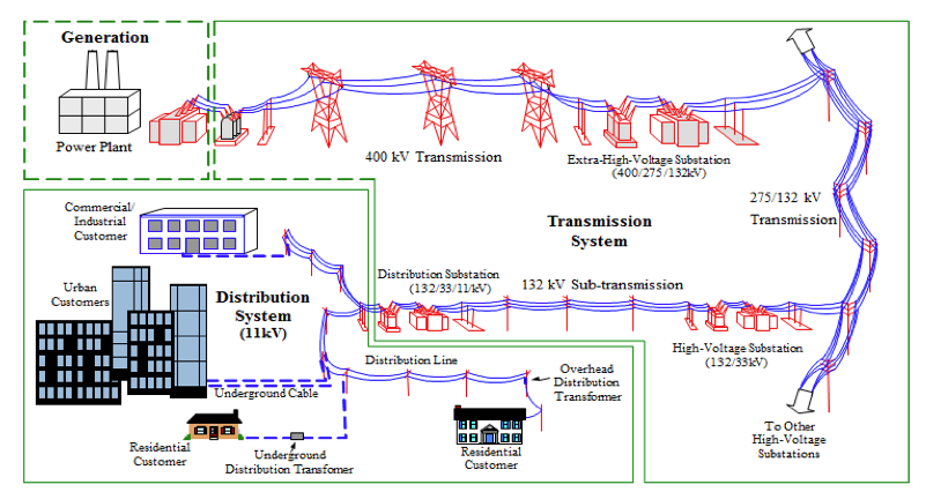
\includegraphics[width=.9\linewidth]{images/DN/HighMediumLowV.png}
    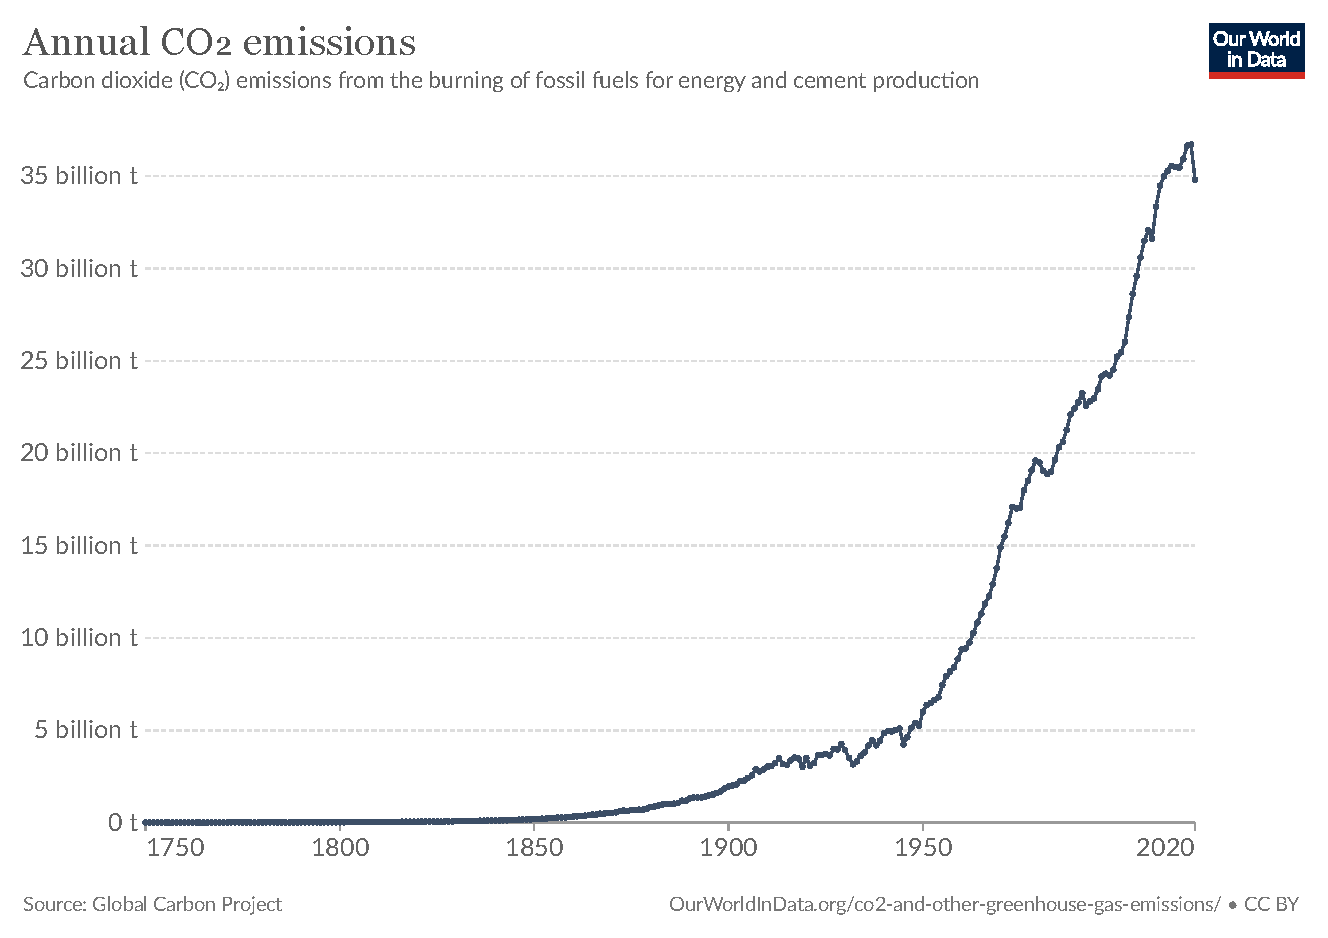
\includegraphics[width=.6\linewidth]{images/Introduction/annual-co2-emissions-per-country.pdf}
\caption[\gls{CarbonDiox} production over the years]{World \gls{CarbonDiox} production over the years \cite{C02prod}}
\end{figure}

Thanks to this emerging trend of decarbonization, more and more renewable power energy devices are introduced in the distribution networks \cite{owidenergy}. With the advantages of inexhaustibility and low impact on the environment, the high penetration of these renewables devices bring in some technical complications for the distribution of power and voltage in the grids. \\
The networks, that have been designed around the conventional centralized energy production, have to adapt to the new generators in the system. It is possible to say that the distribution networks are moving from unidirectional power flow (from the distribution system to the consumers) to a bidirectional power flow (in this case the consumers are also producers and the exceed energy can be transported from the consumers to the distribution system. They are also known as prosumers \cite{prosumers}). This switch from unidirectional to bidirectional power flow requires a smarter system that can handle in an efficient way the generation and distribution of voltage.\\

In the literature, this smarter way to control a distribution system is known as active network management (\gls{ANM}) and it refers to the design of control schemes that modulate the generators, the loads, and the distributed energy storages (\glspl{DES}), as well as other elements like switches, connected to the grid. \\


\section{Aim of the thesis}
\label{sec:aimthesis}
The aim of this thesis is to exploit data-driven approaches to forecast the future distribution of voltages based on historical measurements in a medium-voltage distribution system using machine learning techniques, in particular deep learning models. Predicting over voltages problems in the network would allow avoiding possible consequences related to these issues. Moreover, some control voltage techniques will be employed to avoid the critical network situation, like for example over voltages problems.

% \section{Research methods}

\section{Thesis outline}
% Chapter 2 provides
% \\
% Chapter 3 ...


\chapter{Background}
%https://www.researchgate.net/figure/A-bidirectional-system-with-distributed-generation_fig2_286569839
%This section gives an overview of the conducted research work to provide a central theme for the reader of this doctoral thesis. This overview should help to understand each individual paper in the annex, representing essential parts of this doctoral thesis, in the overall context of the developed optimization methodology.

The voltage control problem has been studied for years, but it only comes under the spotlight in recent years for the increasing number of distributed resources introduced in the networks. It is important to control the voltage in an electrical power system for a regular operation of the electrical equipment, to prevent damage such as overheating of devices and lines, to reduce transmission losses and to maintain the ability of the system to last and prevent voltage collapse. \\

%https://electrical-engineering-portal.com/how-reactive-power-is-helpful-to-maintain-a-system-healthy
In particular, it is useful and sometimes needed to reduce the output of renewable generators to prevent possible voltage problems. This means that the output power of these generators is less from what they could otherwise have produced given the available resources. Such prevention is often referred to as the process of \textbf{curtailment}. Said generation curtailment, along with storage and transmission losses, constitute the principal sources of energy loss that could be minimised with smart control system like active network management \gls{ANM} \cite{gym-anm}. \\

\noindent Controlling the voltage in an active way has many interesting properties:
\begin{itemize}
    \item It is a combination of local and global problem: the voltage at each node is influenced by the powers of all other nodes, but the impact depends on the distance between them.
    
    \item It is a constrained optimization problem with many constraints, for example to keep the voltage in a given range, and the objective is to minimise the total power loss.
    
    \item Voltage control has a relatively large tolerance, and there are no severe consequences if the control fails to meet the requirements for short periods of time. \cite{wang2022multiagent}
    
    \item It is a hierarchical problem where the information available can be represented as a pyramid: much information is available at the top of the pyramid (distribution stations and substations) and it decreases at the base of the pyramid (houses, factories) mainly due to the absence of many sensors.
\end{itemize}

\section{Power system}
\subsection{Description of a power system}
%https://www.generatorsource.com/Articles/Generator-Info/High-Medium-and-Low-Voltage-Differences.aspx
%Power systems are facilities that produce and transport electricity to consumers. \\
A power system is a complex infrastructure that produces and distribute electricity to different consumers. A power system consists of generation, transmission and distribution system and each of them has a different function. \\

%Power transmission systems consist of an interconnected set of overhead lines, cables and related equipment that are used for the transfer of electricity at high voltage levels between supply points and load points, such as customers and other electric systems. \\

In the traditional power system, electricity is generated in large, centralised power plants. The electricity is then transferred to the loads using the transmission and distribution networks. High and extra-high voltages are associated with supply transmission from the power plant. The reason for transmitting power at high and extra-high voltage levels is to increase efficiency. The lower current accompanying the high voltage transmission allows for the use of thinner, lighter-weight cables. This reduces the cost in the tower and electrical line construction. In Belgium, high and extra-high voltages refer to voltage magnitudes $30 kV \leq |V| < 380 kV$ for the high voltage and $|V| \geq 380 kV$ for the extra high voltage \cite{elia}. (\emph{Symbols problem: V for voltage magnitude and V for volts?})\\
Large industrial complexes and factories that require a substantial amount of power often utilise medium supply voltages. The high voltage coming from the power plant is sent to the primary substation, this can supply step-down power to secondary substations or to single buildings. Secondary substations can have transformers to further step down the power, and they are generally located in areas that can serve one or more buildings. Medium voltages refer to voltage magnitude $0.4 kV \leq |V| < 30 kV$. \\
Then the medium supply power is step down again to a low voltage and sent to the domestic household or home appliances power supply. Low voltages refer to voltage magnitude $|V| < 0.4 kV$. \\
\begin{figure}[H]
\centering
    % 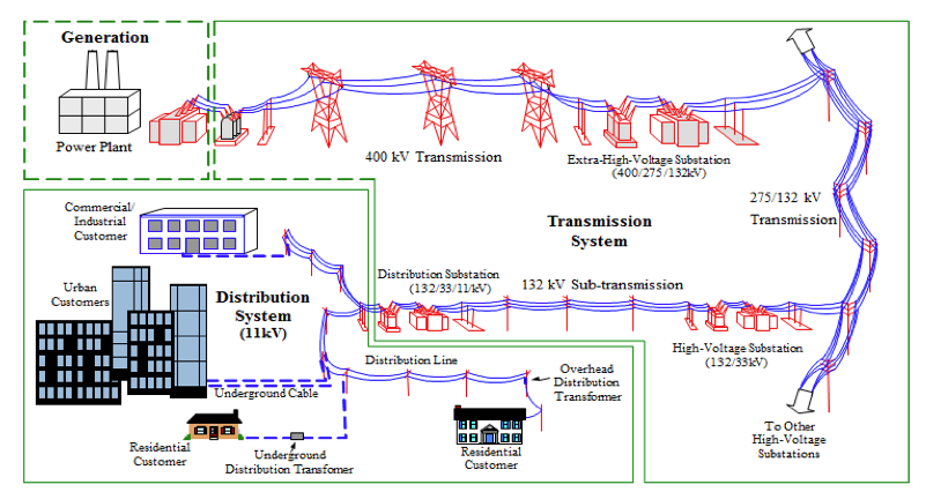
\includegraphics[width=.9\linewidth]{images/DN/HighMediumLowV.png}
    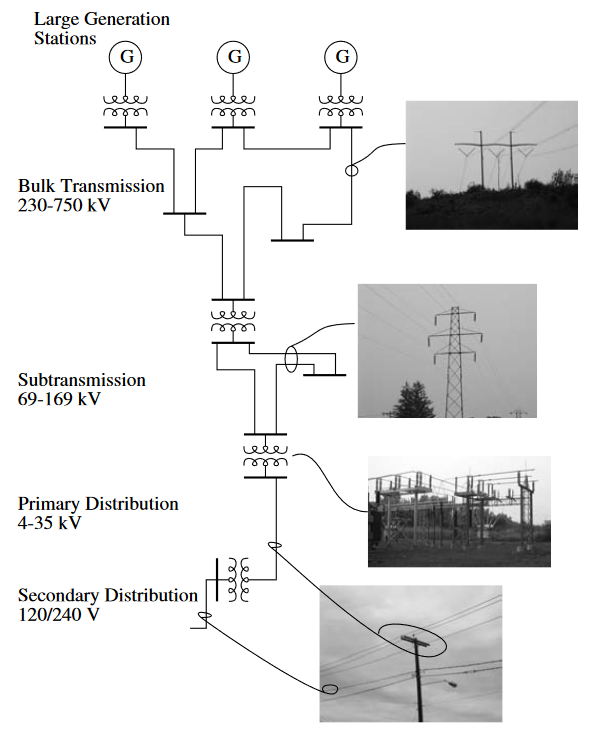
\includegraphics[width=.25\linewidth]{images/Background/DN/DN.PNG}
\caption[Power network distribution]{Power network distribution \cite{EPD}}
% \label{fig:gym_anm_net}
\end{figure}


\noindent A power system is usually made up of the following main elements: \label{networkeledesc}
\begin{itemize}
    \item \textbf{Generator}. These generate energy, converting a form of energy into electricity. In general, electricity is produced when a magnet is moved near a wire to create a steady flow of electrons.\\
    So, many generators produce energy using turbines: a fluid spin the generator's blades, producing electricity. This fluid, either water or air, can derive from natural sources: hydroelectric, wind or geothermal turbines, or generated by combustion of some fuel, for example coal, natural gas, oil or nuclear source. \\
    There are other generators that do not need a turbine to generate electricity, for example solar panels.
    
    \item \textbf{Lines}. These transport the power from where energy is generated to where it is consumed. One of the main issues about transportation lines is insulation. \\
    There are different types of lines: overhead cables, they use air to insulate the bare conductors or underground cables, for these cables particular attention must be taken to insulate them from other conductors and from the earth (ground). Also, the material used must be resistant to damages, corrosion, and it must avoid that the water is being absorbed.
    
    \item \textbf{Transformers}. Transformers are used to interlink systems operating at different voltages. These can increase  the voltage magnitude near a generator power plant or decrease it near the consumptions facilities. \\
    Changing the voltage magnitude allows reducing the power loss due to transportation. One of the main causes of power loss is the Joule effect: some part of the energy transmitted is converted in heat generated by the current flowing through a conductor. This power lost is given by the equation $P=VI$, where \gls{V} is the voltage and \gls{I} is the current, so decreasing the voltage reduces the energy loss.
    
    \item \textbf{Switchgear}. In an electricity supply, it is necessary to disconnect equipment from the network quickly if a fault occurs to avoid damage on the elements of the network, or to disconnect some points of the network to avoid excessive losses or too high or low voltages. \\
    Switchgear is a broad term that describes a wide variety of switching devices that fulfil the need of controlling, protecting, and isolating power systems. Among these switching devices the most common are: \emph{circuit breaker}, during an electrical fault, a circuit breaker will detect the anomaly and interrupt the power flow, effectively limiting damage to the system; \emph{switch} is an electrical component that can disconnect or connect the conducting path in an electrical circuit, interrupting the electric current or diverting it from one conductor to another; \emph{recloser} similar to the circuit breaker but used in high voltage networks, these devices handle trouble temporary occurrences such as lightning, windblown tree branches or wires,
    birds, or rodents damaging the wires.
    
    \item \textbf{Loads} are electric components that consume the electric power generated by power plants. The type of loads can be divided base on the consumption in:
    \begin{itemize}
        \item[] \emph{Domestic loads}, the domestic loads mainly consist of lights, fan, refrigerator, air conditioners, mixer, grinder, heater, ovens, small pumping, motor, etc. The domestic loads consume very little power.
        \item[] \emph{Commercial loads}, the commercial loads mainly consist of lightning, fans, heating, air conditioning and many other electrical appliances used in establishments such as markets, restaurants, shops. This type of load occurs for more hours during the day as compared to the domestic load.
        \item[] \emph{Industrial loads}, the industrial loads refer from a small-scale industry, to a heavy industry. It includes all electrical loads used in industries along with the employed machinery. Industrial loads may be connected during the whole day \cite{EDNdesign}.
    \end{itemize}
    
    \item \textbf{Buses} are nodes where a line or several lines are connected and may also include several components such as loads and generators.
    % \item Load buses where \gls{P} and \gls{Q} are specified.
    % \item Generator buses where the voltage magnitude \gls{V} and the power \gls{P} are specified.
    % \item A primary bus, an "infinite" bus, where the magnitude voltage \gls{V} is specified (normally 1 \gls{pu}) and its phase angle \gls{Vangle} is assumed to be zero as a reference angle. At this bus, both \gls{P} and \gls{Q} can be what is needed to keep the network stable. \cite{eps}
\end{itemize}

\subsection{Power flow}
\label{powerflow}
%Mathmatical formulation: https://www.engineering.iastate.edu/~jdm/ee458_2011/PowerFlowEquations.pdf
%Simple discussion: https://www.pterra.com/power-flow-analysis/power-flow-solution-techniques/
An important procedure in power system networks is to perform a numerical analysis to determine the electrical state of the network, starting from some parameters that are known. This analysis is called power flow (\gls{PF}).\\
%The \gls{PF} is an optimization problem essential for planning purposes: besides the calculation of electrical characteristics of the power system, power flow analysis can also help to optimize the system operating conditions, minimize the power losses and determine control actions to satisfy the demand while meeting operational constraints.

\subsubsection{Buses}
The power flow gives information about the steady state of the entire system such as voltage, active, reactive power and lines' loading.\\
Each bus is associated with four quantities: voltage magnitude \gls{V}, phase angle \gls{angleV}, real power \gls{AP} and reactive power \gls{Q}.
Depending on the quantity that have been specified, buses in the power system are classified into the following three different types:
\begin{itemize}
    \item \textbf{Slack bus}. It is taken as reference where the magnitude and phase angle of the voltage are specified. Slack bus magnitude considers 1 \gls{pu} and phase angle 0 degrees. This bus provides the additional real and reactive power to supply the transmission losses, since there are unknown until the final solution is obtained.

    \item \textbf{Load buses or PQ bus}. At these buses, the real and reactive powers are specified. The magnitude and phase angle of the bus voltage are unknown until the final solution is obtained.

    \item \textbf{Voltage controlled buses or PV bus}. At these buses, the real power and voltage magnitude are specified. The phase angles of the voltages and the reactive power are unknown until the final solution is obtained. The limits on the value of reactive power are also specified. 
\end{itemize}

\subsubsection{Solution techniques}
Defining and solving the power flow equations are the main tasks in load flow analysis. \\
The definition of the power flow equations is based on Ohm’s Law, which is the relationship between voltages and currents. For a network, it can be expressed in matrix notation as follows:
\[
    \mathbf{Y} \times \mathbf{V} = \mathbf{I}
\]
\[
 \begin{bmatrix}
 Y_{1,1} & Y_{1,2} & \quad & \cdots & \quad & Y_{1,N-1} & Y_{1,N} \\
 & & & & & & \\
 Y_{2,1} & Y_{2,2} & \quad & \cdots & \quad & Y_{2,N-1} & Y_{2,N} \\
 & & & & & & \\
 
 \vdots & \vdots & \quad & \ddots & \quad & \vdots & \vdots \\
 & & & & & & \\
 
 Y_{N-1,1} & Y_{N-1,2} & \quad & \cdots & \quad & Y_{N-1,N-1} & Y_{N-1,N} \\
 & & & & & & \\
 Y_{N,1} & Y_{N,2} & \quad & \cdots & \quad & Y_{N,N-1} & Y_{N,N} \\
 \end{bmatrix}
 \times
 \begin{bmatrix}
 V_1 \\ \\ V_2 \\ \\ \vdots \\ \\ V_{N-1} \\ \\ V_N
 \end{bmatrix}
 =
 \begin{bmatrix}
 I_1 \\  \\ I_2 \\ \\ \vdots \\ \\ I_{N-1} \\ \\ I_N
 \end{bmatrix}
\]

\noindent Where:
\begin{itemize}
    \item \textbf{Y} is the bus admittance matrix
    \item \textbf{V} is an array of bus voltages
    \item \textbf{I} is an array of bus current injections (positive value when generation, and negative value when load)
\end{itemize}

The power flow formulation is based on the application of Kirchhoff’s laws to meshed electric networks. The basic concept is that the sum of all flows into each and every node should be equal to zero.\\
The flows are in complex form, they consist of real and reactive components, or \glspl{W} and \glspl{VAR}. That means that if there are n nodes, then there are n complex equations. The resulting system of equations involves non-linear relationships, making the calculations not easy. Solution methods for this system of equations are primarily iterative with the objective of reducing the sum of flows in all nodes to some acceptably small value known as the mismatch tolerance. \\

All these iterative methods follow the same basic concept: they assume starting values for the dependent variables, primarily voltage at nominal voltage magnitude (i.e. 1 \gls{pu}) and zero phase angle; compute new values for those voltages using the nodal network equation or a numerical approximation and repeat until the convergence criteria are met. \\

The solution has to satisfy some network constrains, in particular:
\begin{itemize}
    \item Active and reactive power balance: the sum of the power injections (that can be positive or negative) at each bus must be equal to 0. This, as said, results from the Kirchhoff’s laws.
    
    \item Voltage limits: the voltage magnitude at each bus and the voltage phase difference between two directly connected buses are bounded by some specific values to maintain the system safe.
    
    \item Thermal limits on transmission lines: the flow in each transmission line is limited due to the thermal limit of the conductors.
    
    \item Generators' active and reactive power limits: the generating units have generally a minimum and maximum level of output power.
    
    \item Generator ramping limits: the output power of a generating unit can not be instantaneously increased or decreased. The operator must take into account the ramping limits of the generators.
\end{itemize}

\subsubsection{Convergence}
The \gls{PF} is a non-linear and non-convex numerical analysis, with a large number of constraints (both equality and inequality constraints) and variables (that can be both continuous and discrete). It is therefore a hard problem, whose cost of finding a solution can increase exponentially, particularly with the increasing size of the network. Moreover, there is no guarantee to find the global optimum. \\
When a solution exists, and it is reached, it is said that the network has converged. Convergence is the state when all nodes have met the mismatch tolerance. \\
The main power flow solution methods are:
\begin{itemize}
    \item Gauss-Seidel method updates the voltage one node at a time until all nodes are within the mismatch tolerance.
    
    \item Newton-Raphson method uses a first order expansion of the power flow equations to approach convergence. Generally faster than the Gauss-Seidel method and able to converge to small tolerances. However, the method is prone to the phenomenon of \textbf{divergence}, when mismatches increase instead of decrease from iteration to iteration. This occurs when the solution vector exits outside the feasible solution space at any point during the algorithm. Once outside feasible space, the solution gradient tends to further increase mismatches, leading to solutions that “blow-up” in the numerical sense. This method requires calculating the first order approximation matrix (known as the Jacobian). \\
    Several variations on the Newton-Raphson are in use, including:
        \begin{itemize}
            \item[] Fast Decoupled: separates the loosely linked real and reactive components of the power flow equations in order to speed up solution.
            \item[] Fixed Newton: does not update the first order approximation matrix every iteration to reduce computational burden.
            \item[] Non-divergent power flow: applies a reduction to the Jacobian multiplier whenever the solution appears to exit feasible space. In certain situations, this may prevent divergence, or at least stop it before blow-up.
        \end{itemize}
    \item Interior-Point Newton method forces the solution inside feasible space to avoid divergence. The interior point method uses a second order expansion of the power flow equations as a basis for its algorithm. The method is more computationally intensive than either the Gauss-Seidel or Newton-Raphson, but is less susceptible to numerical divergence.
\end{itemize}

\subsubsection{Divergence}
Divergence is the condition of the power network when the numerical solution can not be found any more due to some possible issues:

\begin{itemize}
    \item the power system is going to “blow-up.”
    \item the power system is in voltage collapse.
    \item the power system is unstable.
    \item the initial conditions defined were bad or poor.
    \item some issues related to software or input data.
\end{itemize}

Divergence of the power flow solution has traditionally been associated with the singularity of the Jacobian matrix. Since some methods require an inverse of the Jacobian as part of its solution algorithm, singularity of the Jacobian means division by zero \cite{eps}.


\subsection{Power system reliability}
\label{sec:psr}
%https://info.ornl.gov/sites/publications/Files/Pub57467.pdf
Reliability of a power system is an important factor concerning the quality of energy supply. \\
Power reliability can be defined as the degree to which the performance of the elements in a system results in electricity being delivered to customers within accepted standards and in the desired amount \cite{MPRPQ}. \\
Reliability indices typically consider such aspects as:
\begin{itemize}
 \item the number of customers;
 \item the connected loads;
 \item the duration of the interruption measured in seconds, minutes, hours, or days;
 \item the amount of power interrupted;  
 \item and the frequency of interruptions.
\end{itemize}

These factors depend on variable such as reliability of individual items of equipment, circuit length and loading, network configuration, distribution automation, and available transfer capacity \cite{EDNdesign}. \\

For reliability purposes, it is important to know the maximum voltage that can be
transferred with transmission lines to meet the anticipated load demand. It is also important to know the levels of power through various transmission lines under certain contingency outage conditions to maintain the continuity of service. Knowledge of power flows and voltage levels under normal operating conditions are necessary in order to determine fault currents and the ensuing consequences on the stability of the system \cite{eps}. \\

\noindent There exists some standards about power system reliability. \\
The International Electrotechnical Commission (\gls{IEC}), IEC TS 62749 \cite{iec}, that states that the energy suppliers and facility managers need to verify the conformity of the energy supplied to:
\begin{itemize}
    \item maximum limits
    \item statistical limits over a week or a year
\end{itemize}
\noindent Under normal operating condition some values must be verified:
\begin{itemize}
    \item during each period of one week $95\%$ of the 10 minutes mean \gls{rms} values of the supply power voltage shall be within the range of $\pm10\%$ \gls{pu} and
    \item all 10 minutes mean \gls{rms} values of the supply voltage shall be within the range $+10\% \/ -15\%$ \gls{pu}
\end{itemize}

The American National Standards Institute (\gls{ANSI}), C84.1-2016 \cite{ansic84}, voltage standards for service voltage limits, for example, are classified as Range A and Range B limits. The voltage between $0.950$ \gls{pu} and $1.050$ \gls{pu} of nominal voltage lies under Range A, and the voltage between $0.917$ \gls{pu} and $1.058$ \gls{pu} of nominal voltage for $240$ \gls{V} service voltage lies under Range B. Note that the voltage can be within Range B for only a short duration and frequency, and thus corrective measures are necessary to constrict.

%Determining power flow requires measurements of some power system conditions; utilities measure a combination of quantities such as voltage magnitude \gls{V}, real power \gls{P} and reactive power \gls{Q} of the elements connected to the network. 

\subsubsection{Reliability criteria}
\label{ssec:n1cri}
The goal of a distribution system operator (\gls{DSO}) is to ensure a reliable system. Unfortunately, a completely reliable electricity supply is not feasible to obtain since it comes at an infinite cost. So, network operators need to determine an acceptable reliability level, by balancing the costs and benefits, where acceptable reliability level means that all the elements in a network have an acceptable voltage range. \\

The European \gls{GARPUR} project (\textbf{G}enerally \textbf{A}ccepted \textbf{R}eliability \textbf{P}rinciple with \textbf{U}ncertainty modelling and through probabilistic \textbf{R}isk assessment) developed reliability management approaches and criteria. One of these criteria used by system operators is the N-1 criterion. \\

The basic principle of N-1 security in network planning states that if a component, for example a transformer or circuit, should fail or be shut down in a network operating at the maximum levels of transmission and supply, the network security must still be guaranteed. This means that the safety of the system is guaranteed and the spreading of the failure is avoided. \\
It is possible that there may be another contingency before restoring the network after the fail of one element, this criterion is known as N-1-1 criterion.  \\

With the increasing of network complexity more than one element may fault, for this reason there exists other levels of reliability, like the N-2 criteria. In this case, even if in the network two components fail, the network security is guaranteed. \\
This N-2 criteria requires much more computational power since, the system operator must calculate what happens to the network for any combination of two fault elements. So, the problem becomes a combination problem, where the possible combination are given by: $N \choose 2$, with $N$ the number of elements in the network. \\

In general, the calculation can be extended to any generic $k$ elements, but the complexity of the problem increases with the value of $k$. Indeed, the possible combination in a N-k contingency are: $N \choose k$, with $2 < k < N$

% \section{Power system voltage managment}

\section{Pandapower}
\label{ch:pandapower}
This thesis project will be developed with the help of Pandapower. \\
Pandapower is a Python based power system analysis tool aimed at automation of static and quasi-static analysis and optimization of power systems \cite{pandapower}. \\
Pandapower is a powerful tool that allows to easily create a model for any power network using customizable predefined data structures, it can solve the \gls{PF} problems, perform the state estimates, topological graph searches and diagnose the system for possible errors.

\subsection{Data structure}
Pandapower is based on a tabular data structure, where every element is represented by a table that holds all parameters for a specific component. It is possible to add more information at the data structure, indeed, after the calculation of the power flow, a result table, which contains the element specific results of the different analysis methods, is added to the structure. \\
The tabular data structure is based on the Python library pandas. It allows storing variables of any data type, so that electrical parameters can be stored together with status variables and meta-data, such as names or descriptions. The tables can be easily expanded and customized by adding new columns without influencing the Pandapower functionality. All inherent pandas methods can be used to efficiently read, write and analyse the network and results data. \\

A Pandapower network is a Python dictionary that holds all information about the network. Most importantly, it includes element and a result tables for each element type, such as line, transformer, switch, loads. The element table holds all input parameters that are specified by the user, while the result table is used to store the results of the power flow calculation. Input and output parameters are identified by the same index in both tables \cite{pandapower}.

\begin{figure}[H]
\centering
    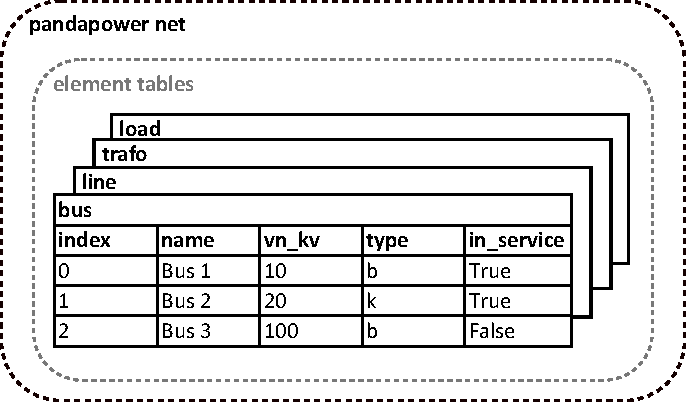
\includegraphics[width=.6\linewidth]{images/Background/Pandapower/Pandapower_net.pdf}
\caption{Pandas data frame representation of the Pandapower network}
% \label{fig:gym_anm_net}
\end{figure}


% \subsection{Network models}
% Pandapower allows to use different type of elements.

% \subsection{Network models}
% There are two main ways of how a power system can be defined by a user.
% A commonly used approach is the bus-branch model (\gls{BBM}), which defines the network as a collection of buses which are connected by generic branches. Branches are modelled with a predefined equivalent circuit and are used to model multiple elements connected to that branch (multi-pole), like lines or transformers. Buses are attributed with power injections to model single-pole elements like loads, generators or capacitor banks. Since the \gls{BBM} is an accurate mathematical representation of the network, electric equations for power systems analysis can be directly derived from it, but the need to calculate the impedances for each branch and to sum power injections at each bus manually can be cumbersome and error-prone, especially for complex elements. \\
% Instead of a \gls{BBM}, Pandapower uses an element-based model (\gls{EBM}) to model electric grids. An element is either connected to one or multiple buses and is defined with characteristic parameters. This allows defining the network parameters, such as length and relative impedance for lines, or short circuit voltage and rated apparent power for transformers. While \gls{BBM} allows only the definition of a summed power injection at each bus, single-pole elements (such as load or generation elements) can be connected to buses independently. This also allows connecting multiple elements at one bus. The element models are then processed internally with the appropriate equivalent \gls{BBM} circuits to derive a mathematical description of the grid \cite{pandapower}. This decoupling the element model from the electric model allows specifying different equivalent circuits for different analysis functionalities. For example, an external grid element can be modelled as a slack node in the power flow calculation, but as a voltage source with internal impedance in the short circuit calculation.

\subsection{Power flow}
The power flow is the most important electric analysis function for power system planning. It allows calculating the current flows and voltages in the network. \\
The Pandapower power flow solver is based on the Newton-Raphson method. The implementation is based on PYPOWER Python library. To solve the \gls{PF}, the bus constraints include maximum and minimum voltage magnitude, active and reactive power limits can be defined for PV and slack-elements like external grids and generators, but also for PQ-elements, such as loads and static generators. \\
% After defining all the network elements, to run the power flow solver it is just need to execute the command: 

% \begin{algorithm}[h]
% \state pandapower.runpp(net, ...)
% \end{algorithm}

After running the power flow calculation, new tables are added to the network data frame.
\begin{figure}[H]
\centering
    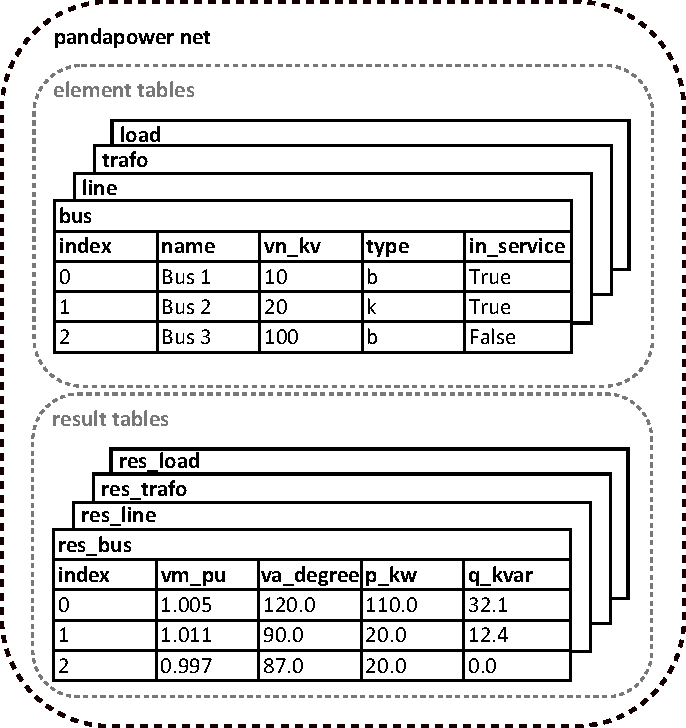
\includegraphics[width=.6\linewidth]{images/Background/Pandapower/Pandapower_resnet_big.pdf}
\caption{Pandas data frame representation of the Pandapower network after the power flow calculation}
% \label{fig:gym_anm_net}
\end{figure}

The power flow calculation on a Pandapower network can fail to converge for a vast variety of reasons, which often makes debugging difficult, annoying and time-consuming. To help with that, the diagnostic function automatically checks Pandapower networks for the most common issues leading to errors. It provides logging output and diagnoses with a controllable level of detail.

%%% SAD :'( %%%
% \noindent this function takes as input the Pandapower network data structure and some other optional values (for example the algorithm solver, max number of iterations, tolerance and so on). \\

% \noindent Internally, Pandapower solves the following optimization problem:

% \begin{align*}
%     \min &\sum_{i \: \in \: gen, sgen, load, external grid} P_i \cdot f(P_i) \\
%         \textrm{s.t.} \\
%         & \text{load flow equations} \\
%         & \text{branch constraints} \\
%         & \text{bus constraints} \\
%         & \text{operation power flow equations}
% \end{align*}

% \noindent where $P_i$ is the active power of any element and $f()$ is the cost function. Few example of the possible constrains are: 
% \begin{align*}
%         & P_{min,i} \leq P_{g} \le P_{max,i}, \; g \in gen \\
%         & Q_{min,i} \leq Q_{g} \le Q_{max,i}, \; g \in gen \\
%         & V_{min,i} \leq V_{g} \le V_{max,i}, \; i \in bus
% \end{align*}

% \noindent It is possible to customize the cost function and choosing between a piece-wise or polynomial cost function. Detailed information about the optimization problem, cost function and network constrains are available in the Pandapower documentation \cite{pandapower2}. \\

\subsection{Time series}
Pandapower allow running time series analysis for a given network. There are two main requirements for time series calculations:
\begin{itemize}
    \item a Pandapower network
    \item some time series (in a panda's data frame for example)
\end{itemize}

To execute the time series calculation, the loads, generators and other elements' active and reactive power time series have to be passed to a controller that will be in charge to change the elements' values according to the time series. \\

The time series calculation can be run with the command: 
\begin{algorithm}[h]
\state pandapower.timeseries.run\_time\_series.run\_timeseries(net, ...)
\end{algorithm}

\noindent this command will start a loop that iterates over every \textbf{time\_step}. For each step, a control loop is started for each controller by \textbf{run\_control}. The controller updates the elements' values at each step with the values given in the time series.

\begin{figure}[H]
\centering
    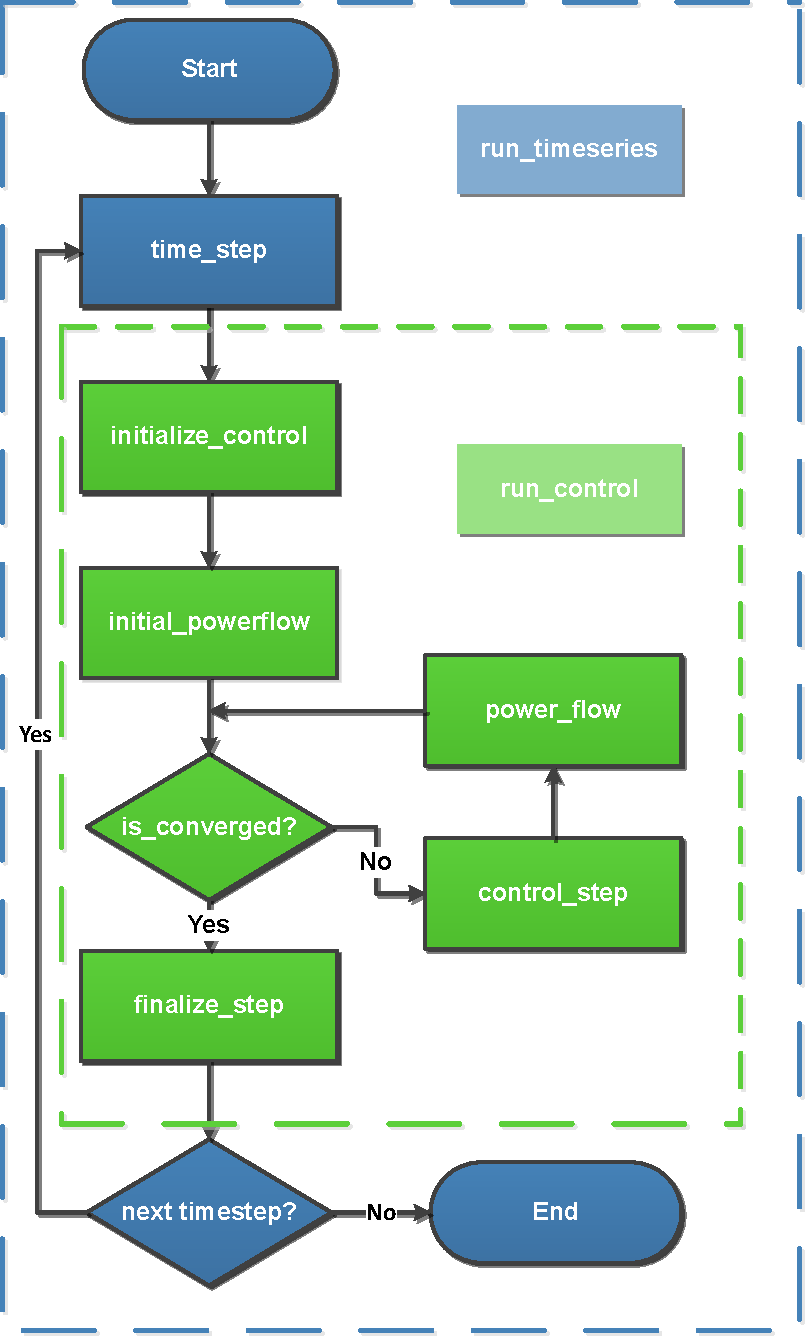
\includegraphics[width=.4\linewidth]{images/Background/Pandapower/run_timeseries_loop.pdf}
\caption{Pandapower time series calculation loop \cite{pandapowerts}}
% \label{fig:gym_anm_net}
\end{figure}

After each step, the elements' values are stored in an output writer object and this allows, after the full calculation is finished, to easily save the values on disk.

\subsection{Other functionality}
Pandapower has some other features:
\begin{itemize}
    \item Predefined Networks. In addition to creating custom networks through the application programming interface (\gls{API}), 66 predefined, published test and benchmark networks can be directly accessed through Pandapower. One of these networks, MV Oberrhein, is the one used in this thesis.
    \item Plotting features. Pandapower comes with extensive plotting features using the Matplotlib library. All Pandapower elements can be translated into different Matplotlib collections that can be customized with respect to shape, size and colour to allow highlighting and create individual network plots. It is also possible to use colour maps to codify information, like the loading of lines or the voltage at buses.
    \item Converter. Pandapower includes converters in order to export a Pandapower grid as a MATPOWER or PYPOWER casefile or the other way.
\end{itemize}



% \section{Machine learning overview}
% \label{sec:ml}
% %https://www.digitalocean.com/community/tutorials/an-introduction-to-machine-learning
% Machine learning is a subset of artificial intelligence that trains a machine to learn. In particular machine learning is the study of how a computer algorithm improves its performances at some task through experience or more precisely:
% \begin{quote}
%     \centering
%     A computer program is said to learn from experience E with respect to some class of tasks T and performance P, if its performance at tasks in T, as measured by P, improves with experience E \cite{mltm}.
% \end{quote}
% \noindent where generally, in a machine learning problem, T is a task too complex to be solved with human written algorithms.\\

% Machine learning differs from the traditional computer science methods.  In traditional approaches, algorithms are sets of explicitly programmed instructions, or rules, used by computers to solve a problem. Machine learning algorithms instead allow for computers to train on data inputs and use statistical analysis in order to output values or answers. \\

% \emph{image with traditional vs ml approaches}\\

% In machine learning, tasks are generally classified into broad categories. These categories are based on how learning is received or how feedback on the learning is given to the system developed.
% There are three main type of machine learning algorithms: supervised, unsupervised and reinforcement learning.

% \subsection{History}
% A brief timeline with the most significant achievements in the machine learning field: \\
% in \emph{1943} Walter Pitts and Warren McCulloch published a paper with the first mathematical modelling of a neural network, taking inspiration from the human biology, Pitts thought as human neuron cell as a threshold logic unit working together with other neurons to build a complex system \cite{McCulloch1943}; in \emph{1950} Alan Turing introduce the Turing Test, a method that tests the machine's ability to show human intelligence \cite{turingtest}; in \emph{1952} Arthur Samuel developed a program on an IBM computer that could play checkers and improve over time; in \emph{1956} the Dartmouth College summer AI conference is considered the birthplace of artificial intelligence where McCarthy coins the term for the first time; in \emph{1957} Frank Rosenblatt deigned the first neural network called perceptron \cite{Rosenblatt1958ThePA} which one year later will be tested on computer, achieving good results, it was able to learn to distinguish right punched card form the left punched cards; in \emph{1963} Leonard Uhr and Charles Vossler described the first machine learning algorithm that could adaptively acquire and modify features and thereby overcome the limitations of simple perceptrons of Rosenblatt; in the same year Donald Michie wrote a program that solved the tic-tac-toe game; in \emph{1970} Seppo Linnainmaa published a paper about the reverse mode of automatic differentiation, later this method will be known as back propagation; in \emph{1980} Kunihiko Fukushima published a paper on neocognitron, a hierarchical multilayer \gls{ANN} that can "learn without a teacher", used for patter recognition tasks, such as digits recognition \cite{neocognitron}; in \emph{1982} Hopfield made popular a type of recurrent neural network \cite{hopfield}; in \emph{1989} Chris Watkins introduce Q-learning, a reinforcement learning algorithm that looks for the best action for a given state; in \emph{1992} Gerald Tesauro developed a program capable of playing the game backgammon; in \emph{1995} were published influential papers on random forest and support vector machines; in \emph{1996} IBM's Deep Blue, a chess-playing program beat the chess champion at that time, Garry Kasparov; in \emph{1996} a team led by Yann LeCun released the MNIST dataset which will be widely adopted for handwriting recognition; in \emph{2006} Geoffrey Hinton coined the term "deep learning"; in \emph{2009} Fei-Fei Li published the ImageNet dataset, a large dataset for image recognition; in \emph{2012} Alex Krizhevsky, Ilya Sutskever, Geoffrey Hinton developed the AlexNet neural network that improved the accuracy of image recognition \cite{alexnet}; in \emph{2014} Facebook publish the DeepFace algorithm to identify individual in photos; in \emph{2016} Google's AlphaGo program beat the strongest Go player at that time; \emph{2019} DeepMind's AlphaStar reaches Grandmaster level at StarCraft II, outperforming 99.8 percent of human players.

% \subsection{Supervised learning}
%https://citeseerx.ist.psu.edu/viewdoc/download?doi=10.1.1.457.4869&rep=rep1&type=pdf
% In supervised learning, the goal is to learn a function that maps an input $\textbf{X}$ to an output $\textbf{Y}$ based on example input-output pairs and applying this learnt function to predict the output of future unseen data. \\

% In a supervised learning problem, the goal is to find a function $f : \textbf{X} \rightarrow \textbf{Y}$, from a sample data $S_n$ composed by pairs of (input, output) points:
% \[
% S_n = ((x_1,y_1),\dots(x_n,y_n)) \in (X \prod Y)^n
% \]
% Typically, $X_i \subset R^n$ and $y_i \subset R$ for regression problems and $y_i$ discrete for classification problems, for example $y_i \in \{0,1\}$ for binary problems. \\

% In the statistical learning settings, an important hypothesis is that the training data is independently and identically distributed (\gls{iid}). from a probability distribution function $P(x,y)$. The goal of the learning is to find a mapping function $f$ that can encode the property of $P(x,y)$ between the inputs x and the output y. \\

% Another important concept is to evaluate how well the function f performs, calculating the error or loss between the predicted values f(x) and the actual value y. This error is evaluated with a loss, or cost, function $L: Y \prod Y \rightarrow R^+$. There are many loss functions depending on the problem and requirements, one example is the mean absolute error (\gls{MAE}) loss function:
% \[
% L(f(x),y)= \frac{1}{N} \sum_{i=0}^{N} |f(x_i)-y_i| 
% \]
% Many supervised learning algorithms consider the minimisation
% of this loss function as an optimisation problem to find the best predictor among all the possible candidate input-output mappings in the solution space $B$. \\

% With the loss function L, the definition of risk of the function f, also called generalization error, must be introduced:
% \[
% R(f) = \int L(f(x),y) dP(x,y). 
% \]
% The objective is to find the function f in $B$ that minimise the generalization error, R(f).

% \subsection{Artificial neural networks}

% \subsubsection{Perceptron}
% \subsubsection{Multi layer perceptron}
% \subsubsection{Convolutional neural network}
% \subsubsection{Recurrent neural network}

% \subsection{Metrics}

% \subsection{Unbalanced dataset}

% \subsection{Splitting dataset}
% \subsubsection{Cross validation}



\chapter{Problem analysis}
\label{chapter4}
%phd report
%https://roadnighttaylor.co.uk/news/what-is-active-network-management/
The principle of active network management \gls{ANM} is to address congestion and voltage issues via short-term decision making policies \cite{ANMQuentin}. \\
\gls{ANM} creates a smarter network infrastructure providing automated control of various components in the network and provides the information needed to ensure that every device performs in an optimal manner. This automated control allows grid companies to avoid reinforcing the network with expensive upgrades, so reducing the costs.
For example, in case of energy generation from the renewable devices higher than what a single line can handle, a grid company, to avoid congestions and possible overvoltages, has three main options:
\begin{itemize}
    \item Replace the existing line with a line that can handle a higher voltage.
    \item Add another parallel line.
    \item Use \gls{ANM}.
\end{itemize}
The first two solution require some infrastructure investment that can be expensive and problematic, especially in the case of overhead or underground lines.\\
The solution with \gls{ANM} does not require construction cost for the grid company; to keep the network working, in this case, the output of the renewable devices can be curtailed to reduce lines' overloading. \\

In these references, \gls{ANM} schemes maintain the system within operational limits by relying on the curtailment of the generator devices, \glspl{PV}, \glspl{WP} and other \gls{DER} devices. \\
Curtailment of renewable energy may be considered as counter-intuitive on the environmental point of view, and it may be considered as last option. Indeed, this process can slow down the switch to clean energy, because of the lost of the curtailed energy. \\

In this mindset, \gls{ANM} could also be used to control flexible loads and reduce the curtailment effects. These flexible loads, also known as virtual batteries, such as water heaters, air conditioning systems, electric vehicles, can be controlled to be turned on if the energy production is higher than the energy consumption so to avoid curtailment on the generators \cite{flexibleloads}. \\
Another way to reduce the energy curtailment is to use Flexible Alternating Current Transmission System (\gls{FACTS}) devices. They offer some
level of power flow control and enhance the transfer capability over the existing network. This flexibility can be utilized for congestion
mitigation and renewable energy integration. Particularly, \gls{FACTS} devices allow controlling all parameters that determine active and reactive power transmission: nodal voltages magnitudes and angles and line reactance. These devices replace the mechanical switches with semiconductor switches allowed much faster response times. One problem with these devices is the cost a system operator should sustain to implement them in the network \cite{facts}.


\section{Network topology}
\label{sec:nt}
A distribution network can be represented as a direct graph $\mathcal{G}(\mathcal{N},\mathcal{E})$, where \gls{N} is a set of positive integers representing the buses (or nodes) in the network, \gls{E} $\subseteq \mathcal{N} \times \mathcal{N}$ is the set of directed edges linking two buses together. The notation \gls{e} $\in \mathcal{E}$ refers to the directed edge with sending bus $i$ and receiving bus $j$. Each bus might be connected to several devices, which may inject or withdraw power from the grid. The set of all devices is denoted by \gls{D} that can be either loads \gls{L} or generators \gls{G}. \\
Several variables are associated with each bus $i \in \mathcal{N}$: a bus voltage $\mathcal{V}_i$, a bus current injection $I_i$, an active power injection $P_i$ and reactive power injection $Q_i$. The complex powers $S_i$, $S_d$ $\in \mathbb{C}$ injected into the network at bus $i$, or device $d$, can be obtained by the relation $S_i = P_i + \mathbf{i}Q_i$ or $S_d = P_d + \mathbf{i}Q_d$. \\
Similarly, variables $I_{ij}$, $P_{ij}$, $Q_{ij}$ and $S_{ij}$ refer to the direct flow of the quantities in branch $e_{ij}$ as measured at bus $i$ \cite{gym-anm}.\\
\emph{I think this part should be somewhere but I am not sure where to put it. Here it looks like it is not properly linked to the previous or following part.}


\section{Problem statement}
\label{sec:ps}
This thesis will focus on \gsl{ANM} and the problem faced by a system operator to maintain the network within its operational limits. In particular, the \gsl{DSO} will evaluate whether in a given moment there will be a voltage problem and to apply (\emph{maybe}) curtailment to generator devices to maintain the voltage inside a safe range.\\

The \gls{DSO} knows some information about the network and several sets of measurements: 
\begin{itemize}
    \item The network topology: the number of lines, buses, loads and the generators, the lines' length, the distance between buses, and the distance between each load and generator from the external grid. Moreover, lines' impedance are known.
    \item The active and reactive power of the loads at each time step (\emph{due to uncertainty, some measure may be missing}).
    \item The type of \gsl{DER} device, their active power for each time step and the maximum power they can generate.
\end{itemize}

%https://arxiv.org/ftp/arxiv/papers/2102/2102.05657.pdf
% Problem formulation
%The time horizon covered in this problem is considered by checking that the system works under the right conditions over a set of $t \in [1,T]$ discrete periods.\\
The \gls{DSO} will consider the behaviour of the network over a set of discrete time steps $t \in {1,2,...,T-1,T}$ with $T \in \mathbb{N}$ and he will predict if the system in a given time step $t+1$ will be in a critical condition, knowing the system information of the previous time steps. In particular, the \gls{DSO} will consider only the $r$ preceding steps. The system critical state $C_{t+1}$ can be formulated as follows: 
\begin{equation} \label{eq:fmapping}
    C_{t+1} = f(S_{t+r-1},S_{t+r-2},\dots,S_{t-1},S_{t})
\end{equation}
\noindent where:
\begin{itemize}
    \item $S_i$ is the state of the system at one generic time step $i$, $S_i \in \mathbb{R}^n$ with $n$ the number of elements.
    \item $f(\,\dots)$ is a forecasting function that maps the input state system to the critical system evaluation $f: \mathbb{R}^{r,n} \mapsto \{0,1\}$.
    \item $C_{t+1}$ is the forecasted value of the system ($C_{t+1} \in \{0,1\}$) stating if the system is critical ($C_{t+1}=1$) or not ($C_{t+1}=0$). 
\end{itemize}

The state of the system is represented by the loads and generators' active and reactive power and/or the buses' voltage magnitude:
\begin{equation} \label{eq:systemState}
    S_t = [V^1_t,V^2_t,\dots,V^{n-1}_t,V^n_t]
\end{equation}
\noindent where $V^i_t$ represents the voltage magnitude at time $t$ for bus $i$.


\section{Solving methodology}
\label{sec:sm}
It is common in time series forecasting problems to use artificial neural networks (\glspl{ANN}) to find a solution, thanks to their capacity to learn an approximate mapping function from the input space to the output space. In this case, the \gls{ANN} will take as input the information from the network, and it will output a binary value, stating if there will be or not a critical situation in the network. \\

Model inputs consist of state variables from time instance $t-r+1$ to $t$. According to \ref{eq:fmapping} and \ref{eq:systemState}, the input can be expressed as a matrix of state variable:
\begin{equation}
  \begin{aligned}
    \text{input} & = [S_{t+r-1},S_{t+r-2},\dots,S_{t-1},S_{t}]\\
        & = 
        \begin{bmatrix}
         V^1_{t-r+1} & V^1_{t-r+2} & \cdots & V^1_{t-1} & V^1_{t} \\
         & & & & \\
         
         V^2_{t-r+1} & V^2_{t-r+2} & \cdots & V^2_{t-1} & V^2_{t} \\
         & & & & \\
         
         \vdots & \vdots & \ddots & \vdots & \vdots \\
         & & & & \\
         
         V^{n-1}_{t-r+1} & V^{n-1}_{t-r+2} & \cdots & V^{n-1}_{t-1} & V^{n-1}_{t} \\
         & & & & \\
         
         V^n_{t-r+1} & V^n_{t-r+2} & \cdots & V^n_{t-1} & V^n_{t} \\
        \end{bmatrix}
  \end{aligned}
\end{equation}

\noindent Given this input, the \gls{ANN} must output binary value stating whether the system is safe or in critical situation at the time step $t+1$. \\

The strategy behind this thesis is to use supervised learning techniques that may extract optimal solutions, decision-making patterns to be applied to the network.

% \section{Problem statement}
% \label{sec:ProbStat}
% [\emph{old}] With the increasing number of renewable energy generators entering the power distribution systems, more and more stress is placed on the networks. This energy produced by the generators can increase the voltage in certain points of the network, causing blackouts or damaging the network's transmission lines. These are interruptions of the energy distribution, and they must be avoided. \\

% A possible solution to this problem is to control the renewable energy generators to produce less than what they could have produced; known as curtailment process. \\
% In a distribution network, there are some information for the elements connected to the grid, like active and reactive power, magnitude voltage value and so on. These values are recorded and expressed as a multi-dimentional time series.\\

% More formally, given the directed graph \gls{G}, at timestamp $t$ it is possible to know the feature $X=[l_p,l_q,b_V,e_L]$ with $l_p$ and $l_q$ are the active and reactive power of each load $l \in \mathcal{L}$, $b_V$ are the buses voltage and $e_L$ are the loadings of the edge connecting 2 buses. It is possible that $X$ is known, or only a subset of it, $X_s \subset X$ is known due to non-fully observability of the network. This $X$ time series dataset will be the input of an artificial neural network \gsl{ANN}.\\
% The problem can be solved as a classification or regression problem: 
% \begin{itemize}
%     \item as a classification problem, the output of the \gsl{ANN} will be a binary value that states if in the next $n$ time steps there will be an over or under voltage problem. For the loss, many loss functions can be used, for example a binary cross-entropy loss function. Given $p(y_i) \in \{0,1\}$ the output probability prediction given the input $x \in X$ (or $x_c \in X_c$) the loss would be calculated as follows: 
%     \[
%     H = - \frac{1}{N} \sum_{i=1}^{N} y_i \log{(p(y_i))} + (1 - y_i) \log{(1 - p(y_i))} 
%     \]
%     where $y_i$ is the real label, $p(y_i)$ is the predicted probability that there will be a voltage problem and N is the number of inputs.
%     \item for the regression problem, the output of the \gls{ANN} will be the voltage forecast for each buses for the next $n$ time steps. Also for this problem, many loss functions can be used, for example a \gls{MAE} loss function, calculated as follows:
%     \[
%     MAE = \frac{1}{T \cdot N} \sum_{t=1}^{T} \sum_{i=1}^{N} |y_{t,i} - \hat{y}_{t,i}|
%     \]
%     where $y_{t,i}$ is the real voltage value at time $t$, $\hat{y}_{t,i}$ is the predicted voltage at time $t$ and $T$ is the number of future time steps to forecast.
% \end{itemize}

% The distribution network used is the MV Oberrhein network from Pandapower and the time series are taken from the Simbench dataset. This database refers to some real distribution networks in Germany in the year 2016; the dataset spans over one year with a $\Delta t$ of 15 minutes (a total of 35,040 time steps).

% \section{Optimization problem}
% This voltage control problem can be formulated as a stochastic problem, where the goal is to minimise the losses while meeting some constraints. In particular, the objective is to minimise the loss $L_g$ of each generator $g \in$ \gls{G} due to the curtailment and avoid not useful transport of energy and other minor energy losses $L_{\epsilon}$ (read: L of epsilon). Moreover, the system has to satisfy the condition of loads demands, that the network is considered safe and the congestion risk of each edge $r_{e_{ij}}$ is less than a given maximum tolerated congestion risk $R_{e_{ij}}$, e.g. {1\%} and that the power generated by each generator $\bar{g}_p$ is less or equal to its maximum installed capacity $g^{max}_p$, and the active and reactive power of the loads ($\bar{l}_p$, $\bar{l}_q$) are in their limits. \\
% Mathematically (\cite{haulogypaper}):
% \[
% min \sum_{g \in G} L_g + L_{\epsilon}
% \]
% subject to
% \begin{equation*}
% \begin{aligned}
% & r_{e_{ij}} < R_{e_{ij}} \qquad & \forall e \in \mathcal{E} \\
% & g^{min}_p \leq \bar{g}_p \leq g^{max}_p \qquad & \forall g \in \mathcal{G} \\
% & l^{min}_p \leq \bar{l}_p \leq l^{max}_p \qquad & \forall l \in \mathcal{L} \\
% & l^{min}_q \leq \bar{l}_q \leq l^{max}_q \qquad & \forall l \in \mathcal{L} \\
% \end{aligned}
% \end{equation*}


\chapter{Project implementation}
\label{chapter5}
The solving methodology described will be applied to a specific test case.
%The project is developed in Pandapower a, Python based, power system analysis tool aimed at automation of static and quasi-static analysis and optimization of balanced power systems \cite{pandapower}.

%GYM-ANM on github, report branch 04/04/2022

\section{MV Oberrhein}
\label{sec:MVober}
%https://ietresearch.onlinelibrary.wiley.com/doi/epdf/10.1049/iet-gtd.2019.1602
The network used for these experiments is the MV Oberrhein network from Pandapower. MV Oberrhein is a real distribution located at Upper Rhine  (German:  Oberrhein),  Germany. This network is a generic 20 kV power system serviced by two 25 MVA HV/MV transformer stations. The network supplies 141 HV/MV substations and 6 MV loads through four MV feeders. The network layout is meshed, but the network is operated as a radial network with some open sectioning points, i.e., redundant lines/cables. This is common in real network: they are meshed but they operate in a radial way.\\
The grid also includes geographical information of lines and buses and is assembled from openly available data.  \\

A representation of the network can is presented in \ref{fig:MVober}. The blue dots represent the buses where load and/or generators are connected and the yellow squares represent the HV/MV substations.
\begin{figure}[H]
\centering
    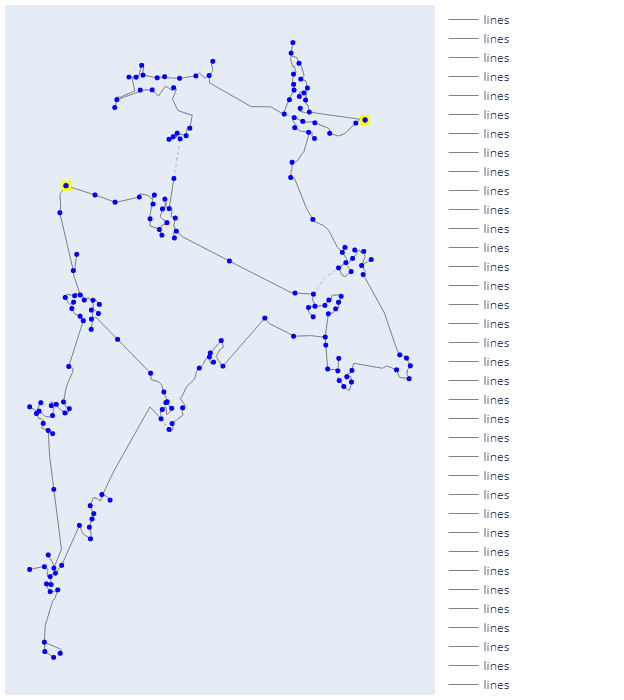
\includegraphics[width=.33\linewidth]{images/MVOberr/Full.png}
\caption{MV Oberrhein network. \emph{add feeders division(?)}}
\label{fig:MVober}
\end{figure}

To simplify the situation, the network can be divided in 2 independent parts [\href{https://kobra.uni-kassel.de/bitstream/handle/123456789/12005/kup_9783737608725.pdf?sequence=1&isAllowed=y}{ref}].

\begin{figure}[h]
\centering
    % 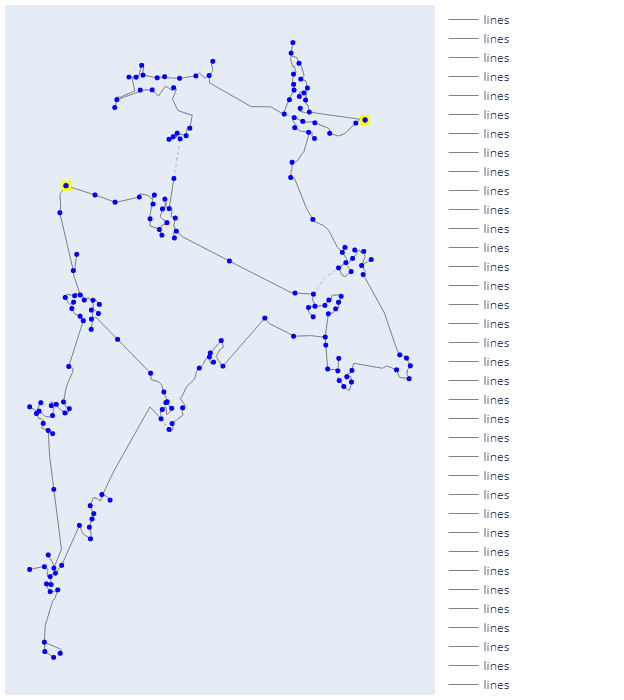
\includegraphics[height=0.33\linewidth,width=.32\linewidth]{images/MVOberr/Full.png}
    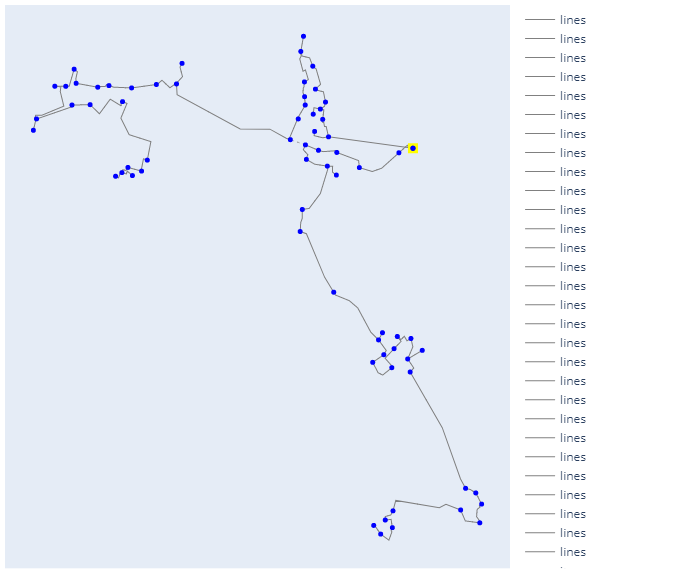
\includegraphics[height=0.33\linewidth,width=.32\linewidth]{images/MVOberr/Half1.png}
    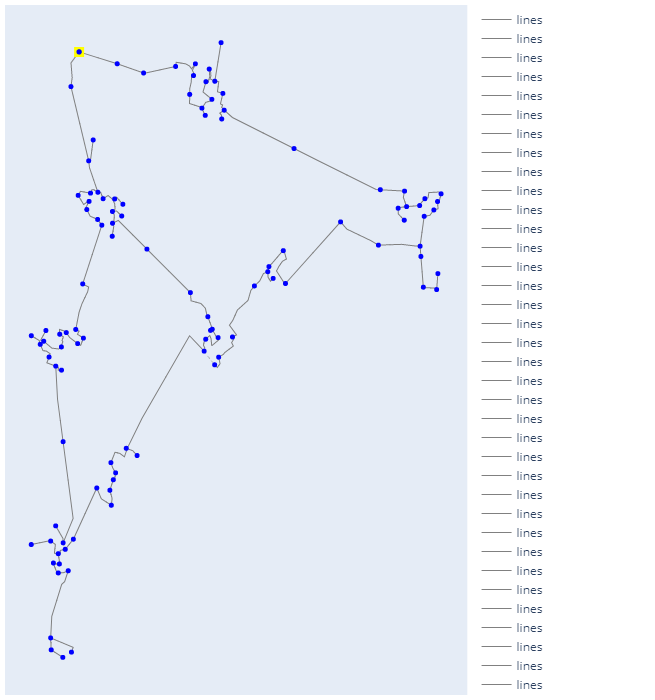
\includegraphics[height=0.33\linewidth,width=.32\linewidth]{images/MVOberr/Half2.png}
\caption{MV Oberrhein network. Used network: middle one \\
TODO add letters}
\label{fig:gym_anm_net}
\end{figure}

The model consist of: one external grid, one transformer, 70 buses, 61 loads and 60 renewable generators.

\subsection{Simbench database}
\label{simdata}
The time series dataset used is taken from the Simbench database. This database refers to some real distribution networks in Germany in the year 2016. SimBench includes multiple time series for one year with 15 min resolution for load, generation and storage units. All time series came as active and reactive power. The time series were grouped by element type, reducing the total number of required time series to a reasonable number, while retaining the possibility to model individual nominal power \cite{Simbenchds0}. All active power values are normalized to the maximum active power value.\\

Power utilities commonly use generic load profiles to group commercial customers with similar load shapes into categories or standard load profiles (\glspl{SLP}). \\
The most commonly used profiles set is developed by the German Association of Energy and Water Industries (\gls{BDEW}). It comprises eleven aggregated profiles, one for residential consumers (H0), three for agricultural (L0-L3), and seven for commercial consumers with different opening hours (G0-G6). They are differentiated into workdays, Saturdays and Sundays as well as three seasonal categories winter, summer, and transitional. The set also includes two profiles for street lightning (B0) and band load (G7). \\
The generation time series for photovoltaics (\glspl{PV}), wind energy and biomass generated for the SimBench dataset are created using the agent-based simulation tool for optimized grid expansion planning SIMONA. SIMONA's power plant models receive real weather data of Germany from the German Weather Service in 2011 for Wind and 2012 for \gls{PV} time series as input data. \\
For 2011 and 2012 generation data, the time axis is adjusted to 2016 by shifting days so that they correspond to the nearest weekday\cite{Simbenchds1}.\\

\begin{figure}[h]
\centering
    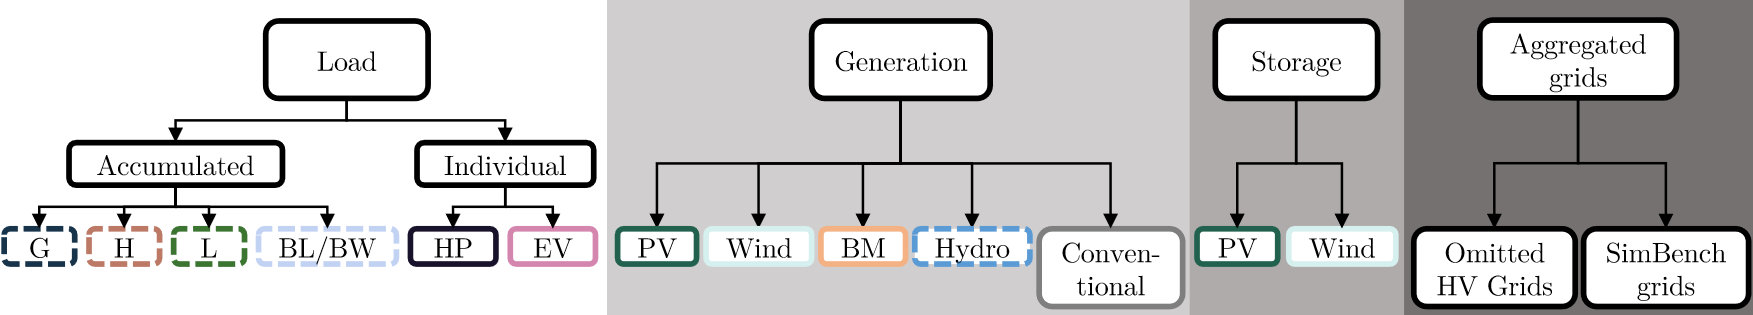
\includegraphics[width=.9\linewidth]{images/MVOberr/SimBench time series types.PNG}
\caption{Overview of the SimBench time series type}
\label{fig:SBtimeseriestype}
\end{figure}

The load time series were distinguished between real measured accumulated, highlighted with a dash, and simulated individual consumers, marked with a solid frame in Figure \ref{fig:SBtimeseriestype}. \\

\subsection{Time series}
\label{ts}
Some time series from the Simbench database are taken to adapt to the number of loads and \glspl{DER} of the MV Oberrhein network in consideration. \\

As said, each element (load or generator) falls under a specific profile type that represent the consumption or generation over time.

\begin{figure}[H]
\centering
    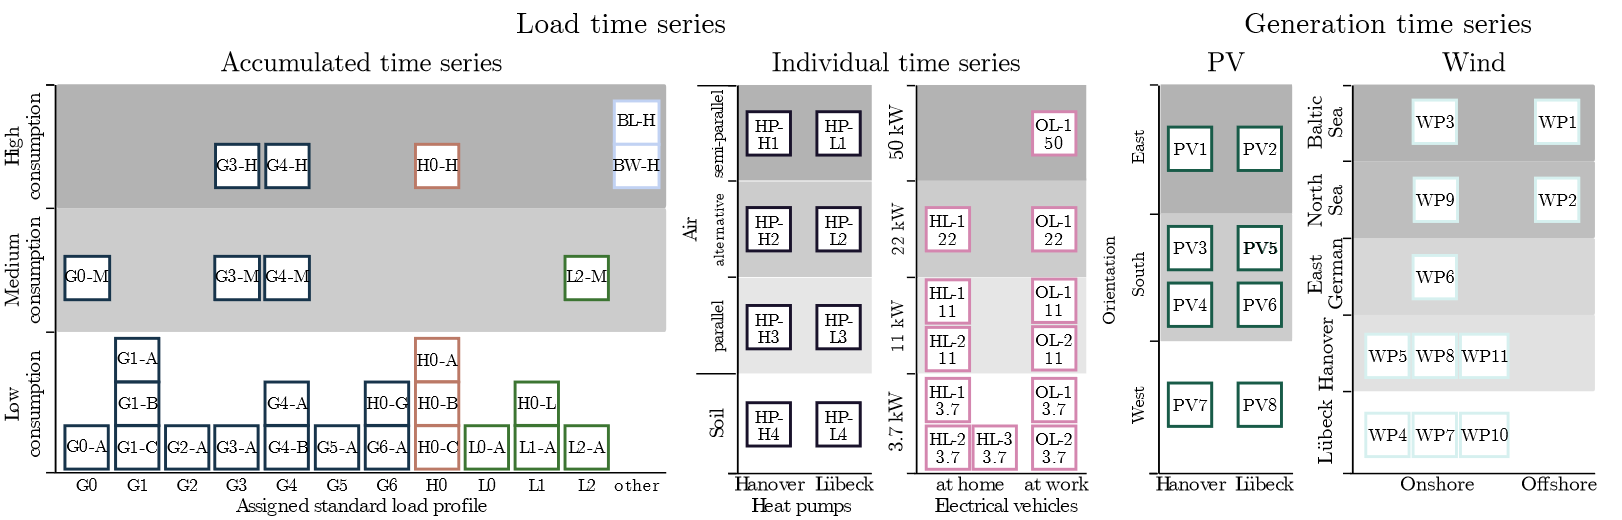
\includegraphics[width=.9\linewidth]{images/MVOberr/SimBench load and generation time series.PNG}
\caption{Load and generations profiles}
\label{fig:gym_anm_net}
\end{figure}

In this case, the profile's types for loads and \gls{DER} are chosen so that every profile type is present to have a network as close as possible to a real network. \\
The profiles' distribution in the Pandapower network is as follows:

\begin{algorithm}[h]
\State Load elements by type: \{{'G3-A': 2, 'H0-L': 3, 'G2-A': 5, 'G3-M': 2, 'G5-A': 2, 'L1-A': 3, 'L0-A': 2, 'H0-C': 6, 'H0-G': 3, 'G1-B': 2, 'G0-A': 4, 'L2-A': 2, 'L2-M': 3, 'G1-C': 2, 'G6-A': 3, 'G0-M': 3, 'G1-A': 3, 'G4-B': 2, 'H0-B': 3, 'G4-A': 3, 'H0-A': 3\}}
\State RES elements by type: \{'WP4': 6, 'PV5': 8, 'PV8': 8, 'PV1': 6, 'PV7': 6, 'PV3': 7, 'PV6': 6, 'PV4': 7, 'WP7': 6\}}
\end{algorithm}

\noindent where the letters stand for: commercial enterprises (G), households (H), agricultural holdings (L) and industrial companies (BL/BW)'; with last letters –A to C indicating low consumption, -M medium consumption, and -H high consumption customers. \\
For the \gsl{DES} device there are photovoltaics \glspl{PV} and wind parks \glspl{WP}. It is possible to notice a bigger presence of \glspl{PV} over \glspl{WP}.\\
% It is important to mention that the \gls{DES} devices are considered as static generators (sgen)

The loads and \glspl{DER} are chosen so that different profile types are present.

\begin{figure}[H]
\centering
    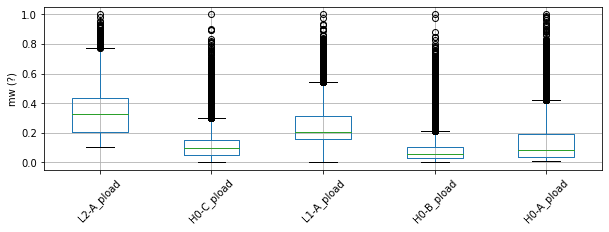
\includegraphics[width=.8\linewidth]{images/MVOberr/BoxPlotLoad.png}
    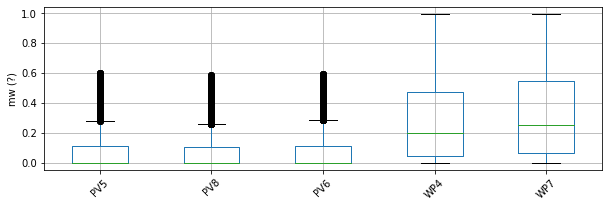
\includegraphics[width=.8\linewidth]{images/MVOberr/BoxPlotRes.png}
\caption{Box plots of load and generation for each profile type}
\label{fig:gym_anm_net}
\end{figure}

Since the profiles are similar for every element of the same type, some noise is added to increase randomness. In particular, the noise added is a scaling factor in the range [0.85,1.15]. The scaling factor allows avoiding negative values in case of a value lower than 1; subtraction may result in a negative value of reactive power for a particular load. \\

\subsection{Partial observability}
To simulate the partial observability problem, some time series are considered as unknown: for just some sparse time steps (missing values) or not available at all. \\

In particular, $x_1\%$ values are randomly selected and set as \emph{NAN} and $x_2\%$ time series of some devices are completely deleted.\\
\emph{Q: Any realistic value for $x_1$ and $x_2$? \label{q:partialobvals}} \\

\noindent These missing values are reconstructed as follows:
\begin{itemize}
    \item for the \emph{NAN} case, it is possible to fill the missing values with the preceding available value. This method, even if simple, is efficient for some reasons: the $\Delta t$ considered is not too large, so it is plausible to expect that loads and generators' values do not change rapidly; it is easy to compute with respect to more complex methods; using only past values allows not to wait for the future values, waiting for the future values may not be acceptable after a deployment of the model.
    
    \item For the case of time series not available at all, it is possible to use balancing flow techniques or generative models like for example \gls{GAN}.\\
    \emph{Q: in this case, isn't a bit overkilling using such method when the load and generator's profile are equal/similar? \label{q:gan}}
\end{itemize}

\subsection{Processing}
For this case, the information used to build the dataset is the voltage magnitude at each buses. The time series will be divided in windows of length, $h$ for the inputs $\textbf{x}$ and length $n$ for the outputs $\textbf{y}$. \\

It is possible to define $\textbf{x}$ as follows:

\begin{equation}
  \begin{aligned}
    \textbf{x}  = 
        \begin{bmatrix}
        V^1_{t-h+1} & V^1_{t-h+2} & \cdots & V^1_{t-1} & V^1_{t} \\
        & & & & \\
        
        V^2_{t-h+1} & V^2_{t-h+2} & \cdots & V^2_{t-1} & V^2_{t} \\
        & & & & \\
        
        \vdots & \vdots & \ddots & \vdots & \vdots \\
        & & & & \\
        
        V^{n-1}_{t-h+1} & V^{n-1}_{t-h+2} & \cdots & V^{n-1}_{t-1} & V^{n-1}_{t} \\
        & & & & \\
        
        V^n_{t-h+1} & V^n_{t-h+2} & \cdots & V^n_{t-1} & V^n_{t} \\
        \end{bmatrix}
  \end{aligned}
\end{equation}
\noindent where $V^i_t$ is the voltage level $V$ of bus $i$ at time stamp $t$. \\

\noindent Instead, $\textbf{y}$ can be defined as previously mentioned: 
\begin{equation}
    \begin{aligned}
        \textbf{y} = [C_{t+1},C_{t+2}, \dots, C_{t+n-1},C_{t+n}]
    \end{aligned}
\end{equation}
\noindent where $C_t$ is the condition of the system at time stamp $t$, with $C_t=1$ if the network is in a critical situation or $C_t=0$ if it is in a normal situation. \\

A time step is considered critical when the voltage of at least one of the buses is out of the boundaries $V_i < v^{\text{min}}$ (under voltage) or $V_i > v^{\text{max}}$ (over voltage), where $v^{\text{min}}$ is the minimum acceptable voltage, 0.95 \gls{pu}, and $v^{\text{max}}$ is the maximum one, 1.05 \gls{pu}.

% \subsection{Different cases}
% With a similar approach for adding some noise to the time series, it is possible to easily create different cases, changing the scaling factors.

% \begin{figure}[H]
% \centering
%     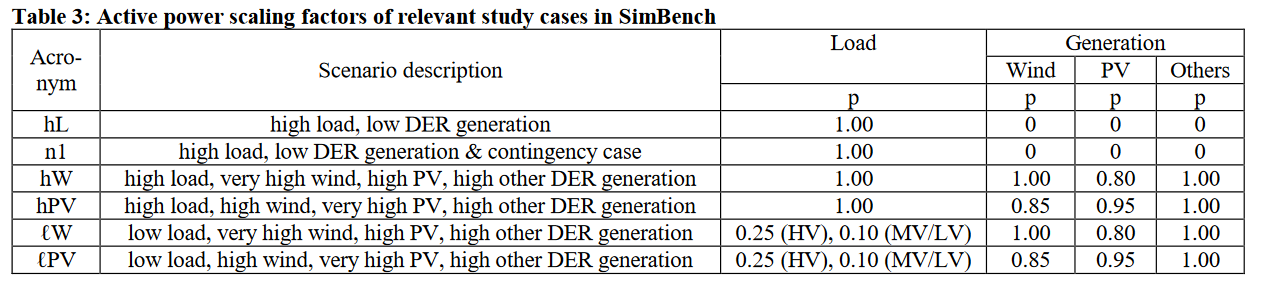
\includegraphics[width=.9\linewidth]{images/MVOberr/Cases.PNG}
% \caption{Possible cases. [\href{https://www.cired-repository.org/bitstream/handle/20.500.12455/526/CIRED \%202019 \%20- \%20139.pdf?sequence=1&isAllowed=y}{ref}] }
% \label{fig:gym_anm_net}
% \end{figure} 



% \begin{figure}[h]
% \centering
%     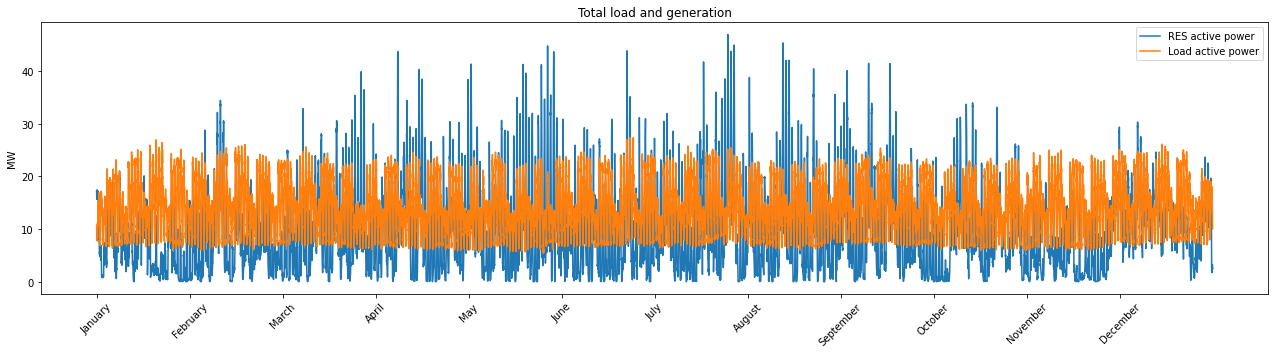
\includegraphics[width=.9\linewidth]{images/MVOberr/Load&Gens.png}
% \caption{Sum of load energy consumption and energy generation over the considered year}
% \label{fig:gym_anm_net}
% \end{figure}

% [old] It is possible to notice a higher consumption of energy over the production, especially at the beginning and end of the year, when the sun intensity is not too high. \\

% \subsubsection{Case: High generation}
\subsection{No partial-observability problem}
As mentioned the time series were normalized so it is possible to use some scaling factors to generate different case. The high generation case refers to scaling factors, as follows:
\begin{algorithm}[H]
    \State {scale\_factor\_load = 1} 
    
    \State {scale\_factor\_sgen = 1.5}
\end{algorithm}

These values are chosen to fit the load and generation profile with the peak capacity of the MV Oberrhein network.

\begin{figure}[H]
\centering
    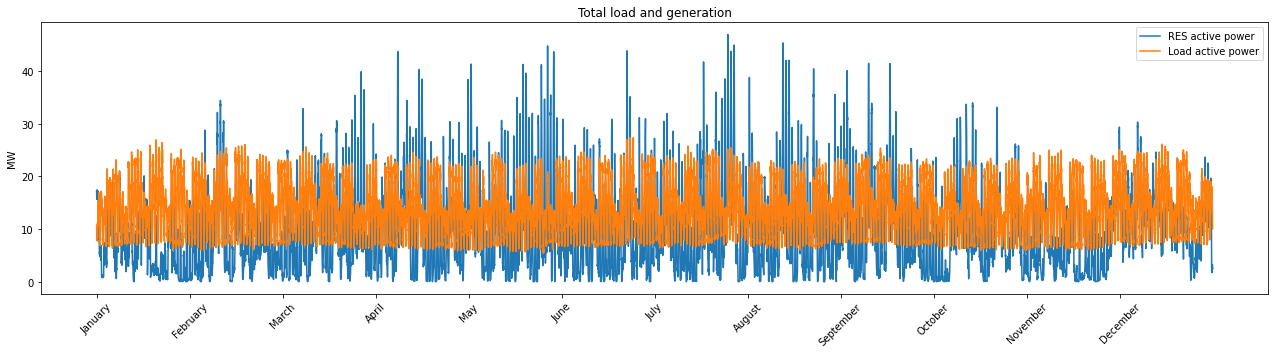
\includegraphics[width=.9\linewidth]{images/MVOberr/Load&Gens.png}
\caption{Sum of load energy consumption and energy generation over the considered year}
\label{fig:gym_anm_net}
\end{figure}

The consumption values are as a typical MV network (\cite{MVnetworks}), while the generation is higher. This case can represent a future power network when the number and the performance of \gls{DER} devices increase, so to have a generation of power higher than the demand; especially during the summer period when the consumption is lower and the generation is higher.\\
Such situation is critical for a network since the surplus energy increase the voltages at the buses that may experience problems or over voltages. \\

% \begin{figure}[h]
% \centering
%     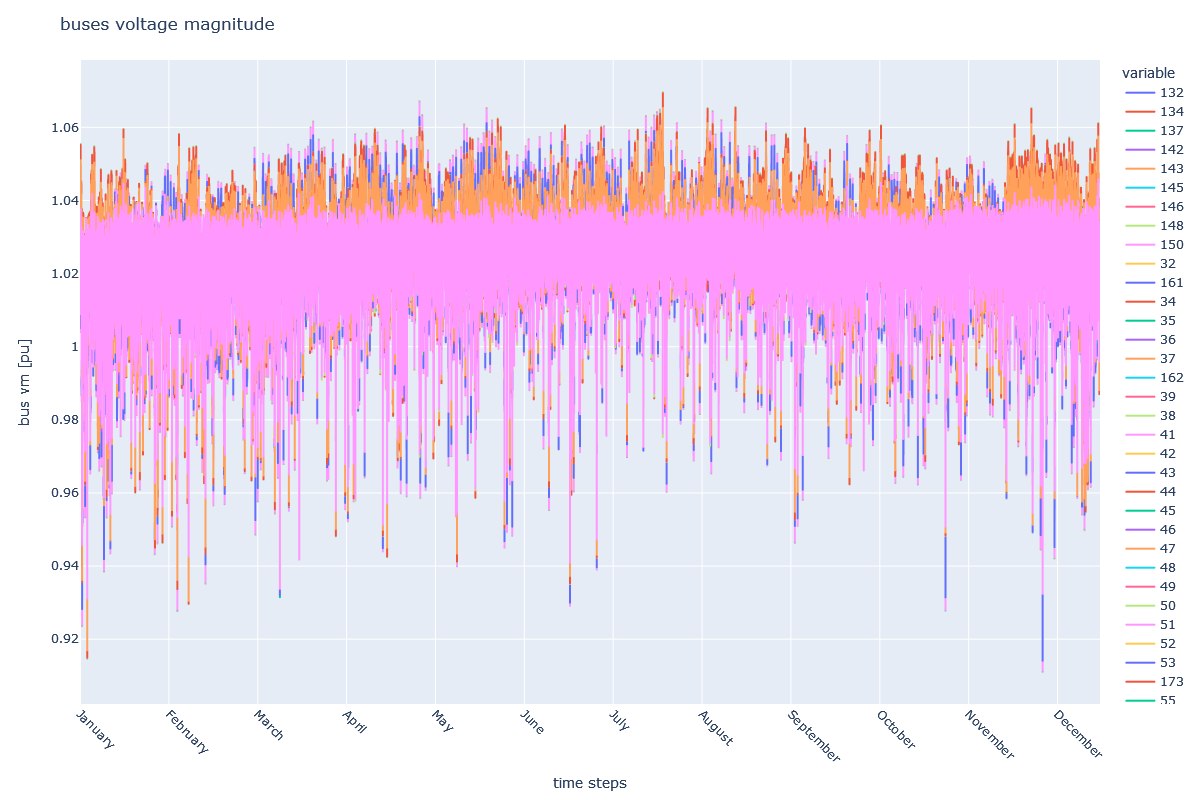
\includegraphics[width=.9\linewidth]{images/MVOberr/High gen.png}
% \caption{Case high generation. Voltage buses results obtained running the time series}
% \label{fig:gym_anm_net}
% \end{figure}

To test whether an over voltage situation occurs or not, the \gls{PF} is calculated using the Pandapower solver.\\
It is possible to see that there are some overvoltage problems. \\
The problems are highlighted in the following plot.

\begin{figure}[H]
\centering
    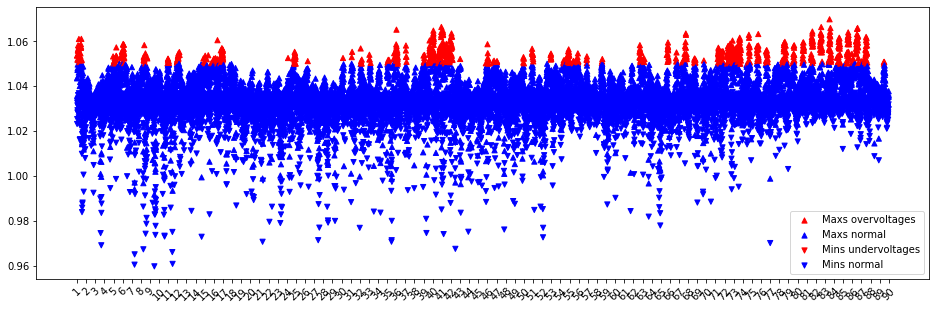
\includegraphics[width=.8\linewidth]{images/MVOberr/CriticalSituation.png}
\caption{In this plot, the maximum and minimum values found for each time step and plotted, so for each time step there are two values representing the highest and lowest value among each bus. The colours, blue and red, represent the normal or critical condition}

 \end{figure}

The full dataset is divided in train, validation and test set with the following proportions: 0.7, 0.2, 0.1 respectively. \\

The dataset is highly imbalanced since the number of times the network is in a critical situation are lower than the number of times the network is under normal situation. This is what usually happens in a power system: networks perform well most of the time and the critical conditions are few.

\begin{algorithm}[H]
    \State Number of critical situations: 1284, over 35040 time steps, ratio: 3.7\% \emph{realistic?}
    \State Number of critical instants in Train set: 646, ratio: 2.6\%
    \State Number of critical instants in Val set: 193, ratio: 2.8\%
    \State Number of critical instants in Test set: 445, ratio: 12.7\%
\end{algorithm}

The data input shape is as follows:

\begin{algorithm}[H]
    \State Inputs shape (batch size, time steps, features): (512, 16, 69)
\end{algorithm}

Three main \gls{ANN} are tested:
\begin{itemize}
    \item \gls{MLP} with two hidden layers of size 192 and 64.
    \item \gls{CNN} with one convolutional layer and one dense layer with 128 neurons.
    \item \gls{RNN} with one \gls{LSTM} as recurrent unit and one dense layer with 128 neurons.
\end{itemize}
All models have as last output layer a fully connected layer whose output size is just one neuron with a Sigmoid activation function.\\

The test are perform considering a temporal window $h$ of 16 time steps (4 hours in the past), while the output window is just one time step in the future (\emph{can be changed to any number}):
\begin{algorithm}[H]
    \State Labels shape (batch size, time steps): (512, 1)
\end{algorithm}

% \begin{figure}[h]
% \centering
%     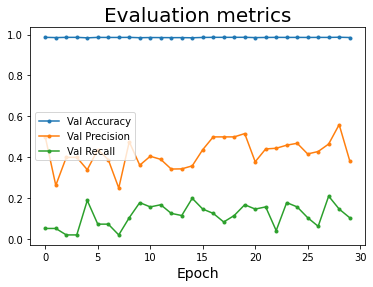
\includegraphics[width=.7\linewidth]{images/MVOberr/DenseNNResult.png}
% \caption{Training history on the validation set for the \gls{MLP} model}
%  \end{figure}

input |V|, h = 16 (4 h) \\
\begin{table}[H]
\centering
\begin{tabular}{l|l|l|l|}
\cline{2-4}
 & \begin{tabular}[c]{@{}l@{}}Test\\ Accuracy\end{tabular} & \begin{tabular}[c]{@{}l@{}}Test\\ Precision\end{tabular} & \begin{tabular}[c]{@{}l@{}}Test\\ Recall\end{tabular} \\ \hline
\multicolumn{1}{|l|}{MLP} & 0.92 & 0.83 & 0.45 \\ \hline
\multicolumn{1}{|l|}{CNN} & 0.89 & 0.55 & 0.93  \\ \hline
\multicolumn{1}{|l|}{RNN} & 0.87 & 0.64 & 0.98 \\ \hline
\end{tabular}
% \caption{}
\label{tab:my-table}
\end{table}


input |V|, h = 4 (1 h) \\
\begin{table}[H]
\centering
\begin{tabular}{l|l|l|l|}
\cline{2-4}
 & \begin{tabular}[c]{@{}l@{}}Test\\ Accuracy\end{tabular} & \begin{tabular}[c]{@{}l@{}}Test\\ Precision\end{tabular} & \begin{tabular}[c]{@{}l@{}}Test\\ Recall\end{tabular} \\ \hline
\multicolumn{1}{|l|}{MLP} & 0.94 & 0.72 & 0.93 \\ \hline
\multicolumn{1}{|l|}{CNN} & 0.90 & 0.56 & 0.99  \\ \hline
\multicolumn{1}{|l|}{RNN} & 0.95 & 0.76 & 0.94 \\ \hline
\end{tabular}
% \caption{}
\label{tab:my-table}
\end{table}



input RES p, h = 16 (4 h) \\
\begin{table}[H]
\centering
\begin{tabular}{l|l|l|l|}
\cline{2-4}
 & \begin{tabular}[c]{@{}l@{}}Test\\ Accuracy\end{tabular} & \begin{tabular}[c]{@{}l@{}}Test\\ Precision\end{tabular} & \begin{tabular}[c]{@{}l@{}}Test\\ Recall\end{tabular} \\ \hline
\multicolumn{1}{|l|}{MLP} & 0.87 & 0 & 0 \\ \hline
\multicolumn{1}{|l|}{CNN} & 0.87 & 0.49 & 0.47  \\ \hline
\multicolumn{1}{|l|}{RNN} & 0.87 & 0 & 0 \\ \hline
\end{tabular}
% \caption{}
\label{tab:my-table}
\end{table}


input RES p, h = 4 (1 h) \\
\begin{table}[H]
\centering
\begin{tabular}{l|l|l|l|}
\cline{2-4}
 & \begin{tabular}[c]{@{}l@{}}Test\\ Accuracy\end{tabular} & \begin{tabular}[c]{@{}l@{}}Test\\ Precision\end{tabular} & \begin{tabular}[c]{@{}l@{}}Test\\ Recall\end{tabular} \\ \hline
\multicolumn{1}{|l|}{MLP} & 0.87 & 0 & 0 \\ \hline
\multicolumn{1}{|l|}{CNN} & 0.87 & 0.12 & 0.002  \\ \hline
\multicolumn{1}{|l|}{RNN} & 0.86 & 0 & 0 \\ \hline
\end{tabular}
% \caption{}
\label{tab:my-table}
\end{table}
% I also tried to add some class weights for the less present class, set bias weights in the last fully connected layer, applied differencing method (subtract time step value at time $t$ with the value at time $t+1$; this removes the time dependency and stabilize the mean. Trend and seasonality are reduced in this way) but the results were still not acceptable.\\

\noindent \emph{Any suggestion? \\ Moreover, what would be an acceptable level of recall/precision/accuracy? I was thinking that since the network can handle a critical situation for some time, if the DSO would curtail some generators, these values should be >0.8 so that it makes sense to trust the model and apply some action.} \label{q:evaluation}

% \newpage
% \subsubsection{Case: High load}
% The high load case refers to scaling factors, as follows:
% \begin{algorithm}[h]
%     \State {scale\_factor\_load = 1} 
    
%     \State {scale\_factor\_sgen = 0.1}
% \end{algorithm}

% \begin{figure}[h]
% \centering
%     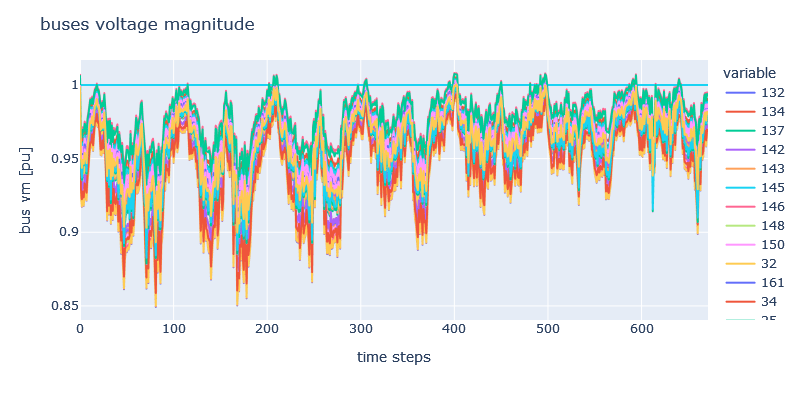
\includegraphics[width=.7\linewidth]{images/MVOberr/High load.png}
% \caption{Case high load. Voltage buses results obtained running the time series}
% \label{fig:gym_anm_net}
% \end{figure}

% In this case, there are only under voltage problems. \\
% The problems are highlighted in the following plot.

% \begin{figure}[h]
% \centering
%     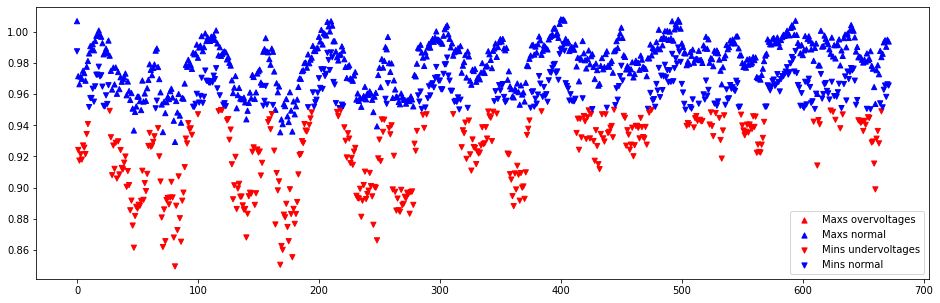
\includegraphics[width=.8\linewidth]{images/MVOberr/High load problems.png}
%     \caption{Same as above, the maximum and minimum values found for each time step and plotted, so for each time step there are two values representing the highest and lowest value among each bus. The colours, blue and red, represent the normal or problem condition.}
% \end{figure}
\chapter{Conclusions and further works}
\label{chapter6}
% \chapter{Related work}
OLTC for regulating the voltage, but they are installed in substations (far from the end of the line)

State-of-the-art voltage control strategies:
-reactive power dispatch base on optima power flow,
-droop control based on local voltage and power measurements
% \label{sec:chapter1}
% \chapter{Related work}
OLTC for regulating the voltage, but they are installed in substations (far from the end of the line)

State-of-the-art voltage control strategies:
-reactive power dispatch base on optima power flow,
-droop control based on local voltage and power measurements
% \label{sec:chapter1}
% \chapter{Related work}
OLTC for regulating the voltage, but they are installed in substations (far from the end of the line)

State-of-the-art voltage control strategies:
-reactive power dispatch base on optima power flow,
-droop control based on local voltage and power measurements
% \label{sec:chapter1}

% \paginavuota % it works even without stile=classica

% \appendix
% % appendix
\chapter{Galileo}
\label{sec:appendix_galileo}

%\lstinputlisting[]{} % for source code files directly
% lstlisting environment for direct inclusion
\begin{lstlisting}[language=Python]
    import os
    os.system("echo 1")
\end{lstlisting}

% for computational complexity
$\mathcal{O}\left(n\log{n}\right)$

% verbatim
\verb+numpy+



% endnotes here if needed

% \paginavuota

\cleardoublepage
\phantomsection
\include{bibliography.bib}
\addcontentsline{toc}{chapter}{References}
\printbibliography

\end{document}
